% Complete documentation on the extended LaTeX markup used for Python
% documentation is available in ``Documenting Python'', which is part
% of the standard documentation for Python.  It may be found online
% at:
%
%     http://www.python.org/doc/current/doc/doc.html

\documentclass{manual}
\RequirePackage[latin9]{inputenc}
\usepackage{graphicx}

\title{AlphaFlow manual}

% Please at least include a long-lived email address;
% the rest is at your discretion.
\authoraddress{
    gocept GmbH \& Co. KG\\
    Forsterstra�e 29\\
    06112 Halle (Saale)\\
    E-Mail: \email{ct@gocept.com}
}

\date{\today}     % update before release!
                % Use an explicit date so that reformatting
                % doesn't cause a new date to be used.  Setting
                % the date to \today can be used during draft
                % stages to make it easier to handle versions.

\release{2.0.0}           % release version; this is used to define the
                          % \version macro

\makeindex          % tell \index to actually write the .idx file

\begin{document}

\maketitle

% This makes the contents more accessible from the front page of the HTML.
\ifhtml
\chapter*{Front matter\label{front}}
\fi

\copyright 2004-2006 gocept gmbh \& co. kg

Licensed under the Zope Public License, Version 2.1 (the ``License''); you may not use this file except in compliance with the License. You may obtain a copy of the License at \url{http://www.zope.org/Resources/ZPL}.

THIS SOFTWARE IS PROVIDED BY THE COPYRIGHT HOLDERS ``AS IS'' AND ANY EXPRESSED
OR IMPLIED WARRANTIES, INCLUDING, BUT NOT LIMITED TO, THE IMPLIED WARRANTIES OF
MERCHANTABILITY AND FITNESS FOR A PARTICULAR PURPOSE ARE DISCLAIMED. IN NO
EVENT SHALL THE COPYRIGHT HOLDERS BE LIABLE FOR ANY DIRECT, INDIRECT,
INCIDENTAL, SPECIAL, EXEMPLARY, OR CONSEQUENTIAL DAMAGES (INCLUDING, BUT NOT
LIMITED TO, PROCUREMENT OF SUBSTITUTE GOODS OR SERVICES; LOSS OF USE, DATA, OR
PROFITS; OR BUSINESS INTERRUPTION) HOWEVER CAUSED AND ON ANY THEORY OF
LIABILITY, WHETHER IN CONTRACT, STRICT LIABILITY, OR TORT (INCLUDING NEGLIGENCE
OR OTHERWISE) ARISING IN ANY WAY OUT OF THE USE OF THIS SOFTWARE, EVEN IF
ADVISED OF THE POSSIBILITY OF SUCH DAMAGE.

\begin{abstract}

\noindent

AlphaFlow is a simple, flexible and easy-to-customize workflow engine for
Plone. It implements an activity based workflow concept to manage content
objects in Plone.

This document is the official documentation for developers and administrators
using AlphaFlow. It contains a tutorial, a user guide and a reference.

\begin{seealso}
    \seetitle[http://www.gocept.com/open\_source\_software/AlphaFlow/]{AlphaFlow homepage}{for up to date news, releases and information about AlphaFlow.}
\end{seealso}
\end{abstract}

\tableofcontents


\chapter{Introduction}

AlphaFlow is an activity-based workflow engine for Plone. It manages tasks to
be performed on content objects. Outstanding features of AlphaFlow are:
\begin{itemize}
    \item a simple workflow definition format
    \item reusable components with exhaustive standard library including
        task assignments, decisions, scripting, email notifications, time based triggers, recursive publication, and more.
    \item easy modelling of complex workflows thanks to decentralized flow
      control
    \item individual workflows for each content object
    \item parallel workflows
    \item flexible management of user assignments as well as permission and
      role mappings for content objects and tasks
\end{itemize}

AlphaFlow is not the only workflow engine available for Zope/Plone. There are two
others:
\begin{itemize}
\item ``DCWorkFlow``, a state-based workflow engine, created at Zope Corporation for use with the CMF.
    DCWorkFlow is integrated into Plone by default.
\item ``OpenFlow'', a general purpose activity-based workflow engine for Zope.
\end{itemize}

Having used DCWorkFlow for a long time and having studied the concepts of
OpenFlow, we are very grateful for those open source systems. AlphaFlow was
built to overcome certain limitations of both engines, but was also build with
the good experiences of DCWorkFlow and OpenFlow in mind.

\section{About this document}

This document is intended to help you get started with AlphaFlow.  It provides
\begin{itemize}
    \item tutorials on how to get started using AlphaFlow and developing with AlphaFlow
    \item an architectural overview
    \item API and library references 
    \item some recipes on standard workflow patterns
\end{itemize}

\section{Terminology}

A real-world workflow is described to AlphaFlow by a ``workflow definition''.
A workflow definition, like a real-world workflow, consists of several steps
which we call ``activities''.

Every time a defined workflow is started, a ``workflow instance'' is created.
The workflow instance runs a series of ``work items''. Each work item
corresponds to an activity. Work items follow up on each other as described by
the workflow definition.

\begin{figure}
  \centering
  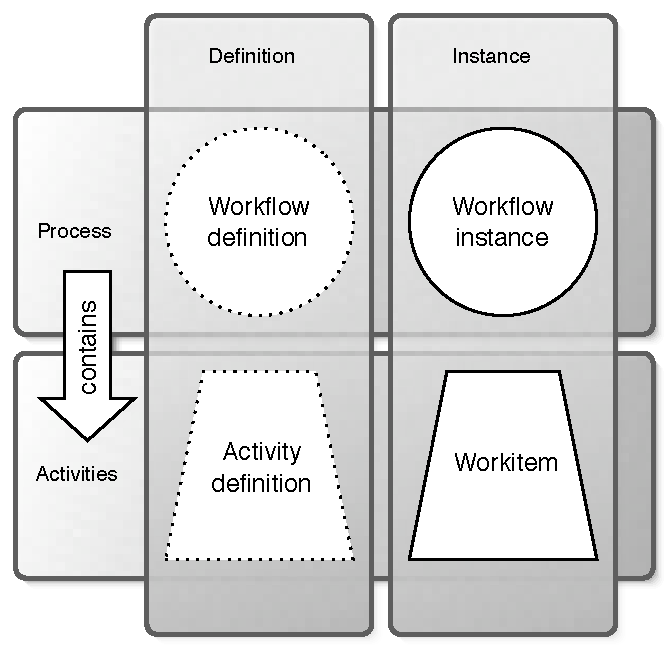
\includegraphics{terminology}
  \caption{\label{fig:terminology}%
    Relationships between a workflow, its definition, and the steps they
    consist of.}
\end{figure}


\chapter{Installation}

AlphaFlow is not hard to install, but if you need help, check the chapter
``Getting support'' on how to get someone to help you.

\section{Prerequisites}

AlphaFlow depends on a couple of software products:

\begin{itemize}
    \item Zope (required: 2.9.6+) -- \url{http://www.zope.org}
    \item Plone (required: 2.5.2+) -- \url{http://www.plone.org}
    \item optional: pygraphviz for visual representations in the workflow
        editor -- \url{http://www.graphviz.org}
    \item optional: PloneTestCase for running the unit tests
\end{itemize}

To develop applications with AlphaFlow you should be familiar with:

\begin{itemize}
    \item the Python programming language
    \item filesystem-based product development for Zope 2, CMF and Plone using Archetypes
    \item a basic understanding of workflow in general
\end{itemize}

\section{Installing}

\begin{enumerate}
  \item Create a new Zope instance.
  \item Put Plone into the \file{Products/} directory.
  \item Unpack the AlphaFlow archive into the \file{Products/}
    directory.
  \item Start the Zope server.
  \item Create a new Plone site.
  \item Install AlphaFlow and (optional: the Procurement) product via QuickInstaller.
\end{enumerate}

After successfully installing AlphaFlow you will find three new objects in
your Plone site: \samp{workflow\_manager}, \samp{workflow\_editor}, and
\samp{workflow\_catalog}. Additionally, AlphaFlow has added a skin layer that
customizes Plone's user interface for AlphaFlow.

\subsection{Installing support for time based activities}

If you want to use time based triggers, like the alarm activity,  you have to
set up an external trigger mechanism, typically a combination of cron and wget.
An example crontab entry to check for triggers every hour looks like this:

\begin{verbatim}
0  *  * * *     wget -S -O - http://<zopeserver>:<zopeport>/<plonesite>/workflow_manager/pingCronItems
\end{verbatim}

You might want to call the trigger more often, based on the time resolution your application needs.

\subsection{AlphaFlow support for the standard content types}
\label{sec:install-patch}

AlphaFlow can only be used with content types that have special properties
which make them AlphaFlow-aware. From Plone 2.1 final on, Plone's default
content types are patched accordingly upon AlphaFlow installation.

To avoid patching the default content types, edit the file
\file{customconfig.py} in the \file{Products/AlphaFlow} directory to read:

\begin{verbatim}
# Only for Plone 2.1: Do you want to patch Plone's default content types to
# use AlphaFlow?
PATCH_PLONE_TYPES = False
\end{verbatim}

To use AlphaFlow with Plone prior to version 2.1 final, you need some
additional Plone product that integrates AlphaFlow into your portal. One such
product is the demo application included in the AlphaFlow distribution.

\subsection{Installing the demo application}

If you want to use the demo application, you also should also:

\begin{enumerate}
  \item Copy or link the Procurement product found in AlphaFlow's
    \file{doc/example/Procurement/} directory into the \file{Products/}
    directory.
  \item Restart the Zope server.
  \item Install the Procurement product via QuickInstaller.
\end{enumerate}


\section{Testing}

AlphaFlow comes with a set of unit tests that you might want to run, to see if your 
environment works with AlphaFlow. In your Zope instance directory run:

\begin{verbatim}
bin/zopectl test --dir=Products/AlphaFlow/
\end{verbatim}

This will start the unit test runner and might take a couple of minutes. It will report you
if everything was OK, or if an error occured. As AlphaFlow supports different environments
you might meet several \code{DeprecationWarning} messages. This is ok, as long as the overall output looks like this:

\begin{verbatim}
----------------------------------------------------------------------
Ran 91 tests in 36.945s

OK
\end{verbatim}


\chapter{Tutorials}

%%%%%%%%%%%%%%%%%%%%%%%%%%%%%%%%%%%%%%%%%%%%%%%%%%%%%%%%%%%%%%%%%%%%%%%%%%%%%%
\section{Using AlphaFlow in a default Plone installation}
%%%%%%%%%%%%%%%%%%%%%%%%%%%%%%%%%%%%%%%%%%%%%%%%%%%%%%%%%%%%%%%%%%%%%%%%%%%%%%

AlphaFlow can be used as a drop-in replacement for Plone's own workflow
mechanism and comes with a few pre-defined workflows. One of those implements
the same kind of reviews as the standard Plone workflow.

This tutorial assumes that you use a Plone 2.5 portal with AlphaFlow installed
and the default content types patched to support AlphaFlow.

%%%%%%%%%%%%%%%%%%%%%%%%%%%%%%%%%%%%%%%%%%%%%%%%%%%%%%%%%%%%%%%%%%%%%%%%%%%%%%
\subsection{Selecting a workflow}

First we need to add a new content object that we want to run a workflow for:
\begin{itemize}
\item Add a new document to your portal. Make sure you saved it once.
\item There is now a new object action called ``select workflow''.
\item The old workflow menu now only displays the status and is ``visible'' in the beginning.
\end{itemize}

Now we can start using a workflow:
\begin{itemize}
\item Click on the ``Select workflow'' action. It will display a list of available workflows.
\item On the workflow listing, you get an overview chart by clicking on the workflow
    icon next to each workflow's title. Here is the chart for the ``simple review'':
\begin{figure}
  \centering
  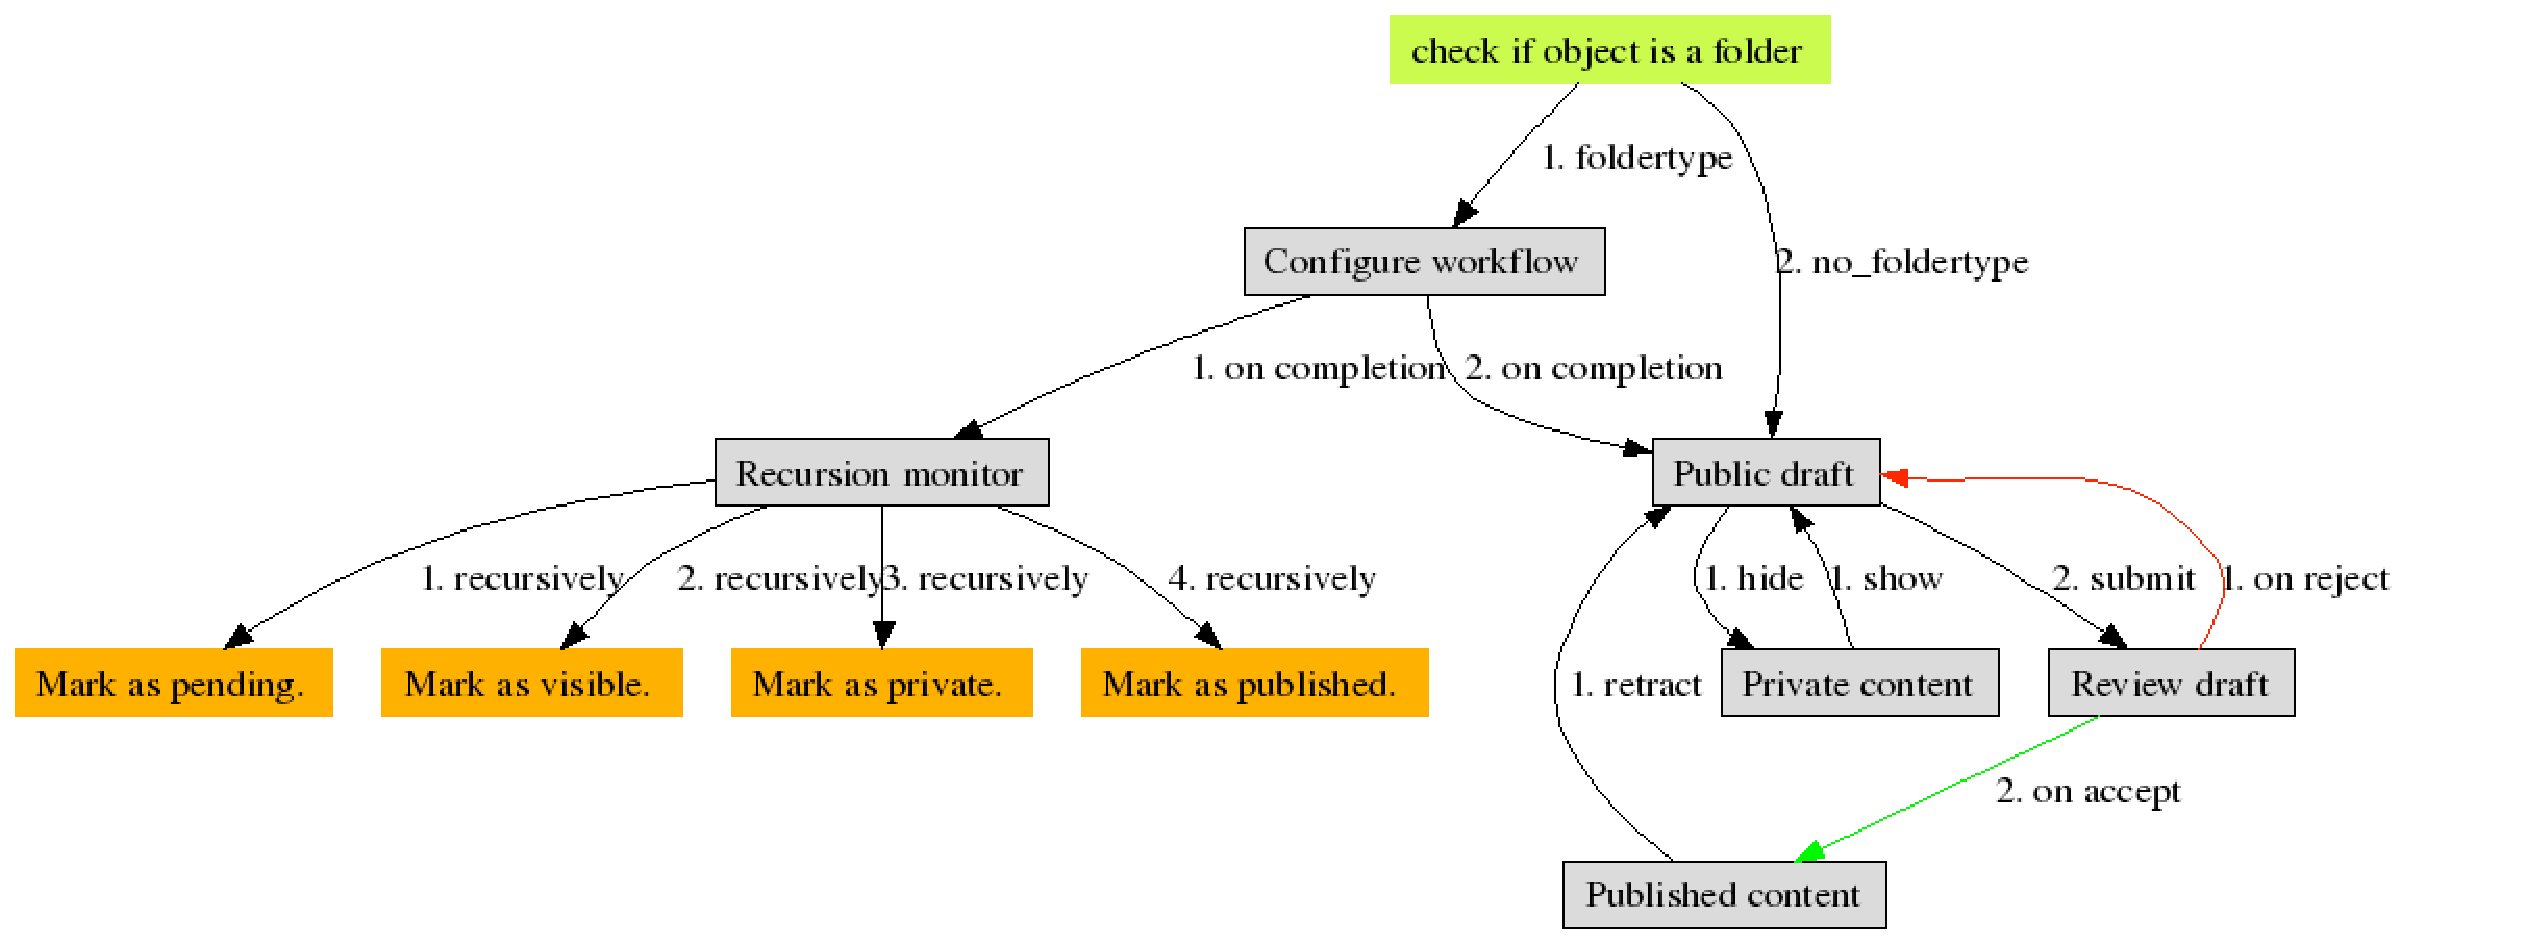
\includegraphics[width=19cm]{simplereview}
  \caption{\label{fig:simplereview}%
    Simple review}
\end{figure}
\item Now, click on the title ``simple review'' to select this workflow for the document.
\item Plone responds with a status message telling you that the workflow has been started.
\end{itemize}

%%%%%%%%%%%%%%%%%%%%%%%%%%%%%%%%%%%%%%%%%%%%%%%%%%%%%%%%%%%%%%%%%%%%%%%%%%%%%%
\subsection{Workflow menu}

After selecting a workflow, the ``workflow menu'' allows everybody involved
with a workflow to perform various operations:

\begin{itemize}
\item Open the workflow menu.
\end{itemize}

The upper part of the menu is titled ``public draft'' followed by three
actions.  You can use the menu to either edit your document in private, submit
it for review or stop the workflow.

In other workflows this menu will have different entries depending on the
actual activities in the workflow.

%%%%%%%%%%%%%%%%%%%%%%%%%%%%%%%%%%%%%%%%%%%%%%%%%%%%%%%%%%%%%%%%%%%%%%%%%%%%%%
\subsection{The work list portlet (``my tasks'')}

When you started the workflow a work item was assigned to you, asking you to
edit the document.  Whenever you have a work item assigned, the portlet ``my
tasks'' will appear and inform you about work items assigned to you. It now
contains the ``write document'' task.

\begin{itemize}
\item Go to the portal home page and follow the link in the work item.
\end{itemize}

You are now back at the document you started the workflow on. The work list
will link you to a relevant page for the work item. In many cases this will be
the content object.

\begin{itemize}
\item Create a new document and also start a ``simple review'' workflow on it.
\end{itemize}

The task portlet has two entries now: one ``public draft'' work item for each
document.

\begin{itemize}
\item Look at the workflow menu of both documents.
\end{itemize}

Both still have only one entry. While the worklist portlet collects all work
items assigned to you on any portal objects, the workflow menu refers to the
work items of the current content object only.

%%%%%%%%%%%%%%%%%%%%%%%%%%%%%%%%%%%%%%%%%%%%%%%%%%%%%%%%%%%%%%%%%%%%%%%%%%%%%%
\subsection{Completing the task}

The workflow menu offers you a list of actions for the ``public draft'' work item. Lets hide the document while we are editing it:

\begin{itemize}
    \item Select the ``hide'' action from the workflow menu.
    \item Enter a comment why we are hiding the document.
    \item Let the action remain on the setting ``hide''.
    \item Click ``submit'' to perform the action.
\end{itemize}

When the work item was completed using the ``hide'' action, the ``simple review'' performed several things:
\begin{itemize}
    \item The workflow status has now changed to ``private''.
    \item The workflow menu now contains a different work item. It is called ``private content''. 
    \item The work list now displays the ``private content'' work item instead of ``edit document.
\end{itemize}

%%%%%%%%%%%%%%%%%%%%%%%%%%%%%%%%%%%%%%%%%%%%%%%%%%%%%%%%%%%%%%%%%%%%%%%%%%%%%%
\subsection{Workflow details}
\label{sec:tut-details}

Now that some things have happened in the workflow, lets look at
the detailed workflow overview.

\begin{itemize}
\item Choose the ``details'' action in the workflow menu of the document you hid
  in the previous step.
\end{itemize}

The details view shows various information:

\begin{itemize}
\item There are two lists of work items, one listing all work items currently
  running, the other reporting on work items already completed. Both show work
  item titles and descriptions and some administrative data.
\item The current list contains one entry for the ``private content'' work
  item which also appears in the workflow menu and the portlet.
\item The history list contains the work item you completed, showing the
  comment you entered for it.
\item The history also lists some work items that were
  run without your interaction when the work flow was started and when you had
  completed the ``public draft'' work item. It is some of those automatic work
  items that updated the DCWorkflow state, others set the permissions on the
  content object as appropriate for making it a public draft or hiding it.
\end{itemize}

%%%%%%%%%%%%%%%%%%%%%%%%%%%%%%%%%%%%%%%%%%%%%%%%%%%%%%%%%%%%%%%%%%%%%%%%%%%%%%
\subsection{Recursive publication of folders}

Working with the rest of the workflow is similar to the first activity. You can
now submit, review and publish it. 

There is another feature of the ``simple review'' workflow worth examining more
closely, though: recursive folder publication and the configuration thereof.

\begin{itemize}
\item Create a new folder in your portal, create some documents and folders
  inside it, and start a ``simple review'' workflow on the folder.
\item A configuration form is displayed.
\item Select the given option for ``recursive publication''
\item Do a series of workflow actions on the folder: hide, show, submit. After
  each, look at objects inside the folder.
\item Notice how the DCWorkflow status displayed is always kept up-to-date
  with the status of the folder itself.
\item Notice also that there is no workflow running on the folder's documents
  and sub-folders. The workflow on the containing folder now affects all
  content objects inside it as well.
\end{itemize}

%%%%%%%%%%%%%%%%%%%%%%%%%%%%%%%%%%%%%%%%%%%%%%%%%%%%%%%%%%%%%%%%%%%%%%%%%%%%%%
\section{Developing an AlphaFlow application}
%%%%%%%%%%%%%%%%%%%%%%%%%%%%%%%%%%%%%%%%%%%%%%%%%%%%%%%%%%%%%%%%%%%%%%%%%%%%%%

Let us introduce AlphaFlow by writing an example application: a procurement
request system. A procurement request system allows you to manage
requests for buying things at your office.
    
On the user's side, some information needs to be entered for each request.
This includes a description of the item to buy, its price, the date it should
be bought, and the relevant account number for your accounting. More data
might be interesting for large scale applications, but this is enough to get a
useful application running.

However, each office using this system will have different rules on who has to
review the request, who is going to buy it, what happens if the request is
rejected, and so on.

This kind of flexibility is made possible by a workflow engine. It adds a
high-level flow control mechanism and allows you to customize the application
to your needs without modifying the application code itself.

\begin{notice}
  All code examples in this tutorial are taken from the code of the example
  application. It can be found in the
  \file{AlphaFlow/doc/examples/Procurement/} directory.
\end{notice}

%%%%%%%%%%%%%%%%%%%%%%%%%%%%%%%%%%%%%%%%%%%%%%%%%%%%%%%%%%%%%%%%%%%%%%%%%%%%%%
% \subsection{TODO A look at the demo application}

%%%%%%%%%%%%%%%%%%%%%%%%%%%%%%%%%%%%%%%%%%%%%%%%%%%%%%%%%%%%%%%%%%%%%%%%%%%%%%
\subsection{Application layout}

The procurement request system is a simple Archetypes application. It provides
two classes which are defined in \file{Procurement/request.py}:
\begin{description}
\item[\class{ProcurementRequest}] an Archetypes object storing the data of
  one procurement request
\item[\class{RequestManager}] an Archetypes folder storing procurement
  requests and providing access to various listings of requests
\end{description}

Procurement requests shall be governed by an AlphaFlow workflow. Therefore,
the \class{ProcurementRequest} class must be AlphaFlow-aware:
\begin{enumerate}
\item The first base class must be \class{AlphaFlowed}:

\begin{verbatim}
class ProcurementRequest(Products.AlphaFlow.public.AlphaFlowed, 
                         Products.Archetypes.public.BaseContent):
\end{verbatim}

\item \class{ProcurementRequest} has to declare that it implements the same
  interfaces as \class{AlphaFlowed} along with the interfaces of the other
  base classes:

\begin{verbatim}
    __implements__ = Products.AlphaFlow.public.AlphaFlowed.__implements__ + \
                     Products.Archetypes.public.BaseContent.__implements__
\end{verbatim}
\end{enumerate}

AlphaFlow allows the application to decide when a workflow is connected with a
content object, and which workflow that is. In our case, each
\class{ProcurementRequest} object is assigned a workflow named
``procurement'' and the instance is run immediately.
    
\begin{verbatim}
    def manage_afterAdd(self, item, container):
        Request.inheritedAttribute('manage_afterAdd')(self, item, container)

        self.assignProcess("procurement")
        self.getInstance().start("Workflow started by request creation.")
\end{verbatim}

\begin{notice}
  The code examples use a more verbose form of referencing class names than is
  used in the actual product code. E.g.
  \class{Products.AlphaFlow.public.AlphaFlowed} will usually be written as
  \class{afapi.AlphaFlowed} in the example product, the AlphaFlow public API
  being imported:
\begin{verbatim}
from Products.AlphaFlow import public as afapi
\end{verbatim}
\end{notice}

In the next step we will define and import a workflow definition.
    
%%%%%%%%%%%%%%%%%%%%%%%%%%%%%%%%%%%%%%%%%%%%%%%%%%%%%%%%%%%%%%%%%%%%%%%%%%%%%%
\subsection{Defining the workflow}

Now we construct a workflow which will handle procurement requests. We will
start with a simple process and evolve it to a more complex setup, introducing
several AlphaFlow features along the way.

\subsubsection{An empty workflow definition}

Workflow definitions are written in an XML syntax called ALF. The XML
definition of the workflow governing our procurement requests starts out like
this:

\begin{verbatim}
<?xml version="1.0" encoding="utf-8"?>

<workflow id="procurement"
          title="Simple Procurement"
          description=
    "A procurement is requested, decided upon and possibly carried out.">

</workflow>
\end{verbatim}

Some comments about the anatomy of this file:
\begin{enumerate}
\item The root element of every ALF file is \member{workflow}.
\item To suggest an id for this workflow definition, the \member{id} attribute
  can be set.
\item The attributes \member{title} and \member{description} characterize
  each process in the user interface.
\end{enumerate}
            
\subsubsection{Adding an activity}

AlphaFlow knows several kinds of activities for describing different steps of
a workflow. We represent the task of writing a procurement request by the
\member{task} activity. Tasks can be assigned to users. After a user has
completed a task, more activities are started. Our workflow definition now
reads:

\begin{verbatim}
<workflow id="procurement"
          ...
          startActivity="edit">

  <task id="edit"
        title="Edit a procurement request"
        completion_activity="review">

    <assignees kind="actual"
               expression="python:[request.Creator()]" />
  </task>

</workflow>
\end{verbatim}

Notes:
\begin{enumerate}
\item The attribute \member{startActivity} of the \member{workflow} element
  lists activities that are started at the beginning of the workflow.
\item Every activity must have an \member{id} so it can be referenced within
  the workflow definition, e.g. as a starting activity.
\item If a \member{title} is given, it appears in the user interface.
\item \member{completion\_activity} lists the activities to be started after
  the user has completed the task. The \member{review} activity will be added
  in the next step of the tutorial.
\item Users are assigned a task by adding the \member{assignees} element to
  the workflow definition. We select the creator of the procurement request by
  specifying a TALES expression.
\end{enumerate}

\subsubsection{Completing the workflow model}

Our workflow involves two more steps: deciding upon the procurement request
made, and buying the item if the request was accepted. The decision whether or not to buy the
requested item requires an activity that supports more than one outcome. 
The \member{decision} activity suits this best:

\begin{verbatim}
  <decision id="review"
            title="Decide whether the article should be bought."
            accept_activity="buy"
            reject_activity=""
            decision_modus="first_yes">

    <assignees kind="actual"
               roles="Finance" />
  </decision>

  <task id="buy"
        title="Buy">

    <assignees kind="actual"
               roles="Procurement" />
  </task>
\end{verbatim}

Notes:
\begin{enumerate}
\item The \member{decision} activity continues with either the activities
  listed in the \member{accept\_activity}, or those listed in the
  \member{reject\_activity} attribute.
\item A decision can be based on input from multiple users. The
  \member{decision_modus} ``first_yes'' means that the request will be
  accepted as soon as any assigned user accepts it.
\item Assignees can be chosen not only by listing their IDs in a TALES
  expressions, but also by giving one or more roles. In that case, all users
  with any of the listed roles are assigned the activity.
\item A workflow can include steps that are not performed within Plone,
  but in other systems or the real world. After the assigned user has bought
  the item, he declares the task ``buy'' completed.
\end{enumerate}

\subsubsection{Emulating DCWorkflow states}

AlphaFlow replaces Plone's own workflow engine, DCWorkflow. It does, however,
not remove it completely. Rather, AlphaFlow uses the fact that DCWorkflow's
states are well integrated with Plone to easily provide the user with
additional information on the progress of workflow instances.

A DCWorkflow state is a label attached to the content object of a given
workflow instance. It is set by the \member{dcworkflow} activity. In our
example, it makes sense to update the DCWorkflow state on completion of each
step in the workflow:

\begin{verbatim}
  <task id="edit"
        ...
        startActivity="dc_private">

  <decision id="review"
            ...
            startActivity="dc_pending"
            reject_activity="dc_rejected">

  <task id="buy"
        ...
        startActivity="dc_accepted"
        completion_activity="dc_bought">

  <dcworkflow id="dc_private"
              title="Mark as private."
              status="private" />

  <dcworkflow id="dc_pending"
              title="Mark as pending"
              status="pending" />

  <dcworkflow id="dc_accepted"
              title="Mark as accepted."
              status="accepted" />

  <dcworkflow id="dc_bought"
              title="Mark as bought."
              status="bought" />

  <dcworkflow id="dc_rejected"
              title="Mark as rejected."
              status="rejected" />
\end{verbatim}

Notes:
\begin{enumerate}
\item The \member{dcworkflow} activity is not assigned to any users. A
  \member{dcworkflow} work item is run automatically as soon as it is created,
  and finishes without waiting for user interaction.
\item The attribute \member{status} is the label to be attached to the content
  object. It may be any string.
\item There are some DCWorkflow states that have special meaning to Plone.
  Among them are ``private'' and ``pending''.
\end{enumerate}

Look at \file{AlphaFlow/doc/examples/Procurement/workflows/minimal.alf} to see
what the final version of the process definition looks like.

%%%%%%%%%%%%%%%%%%%%%%%%%%%%%%%%%%%%%%%%%%%%%%%%%%%%%%%%%%%%%%%%%%%%%%%%%%%%%%
\subsection{Extending the workflow}

In the previous sections of this tutorial, we constructed a procurement
request manager that subjects each request to a straight three-part workflow:
After a request has been created, it is edited by its creator and reviewed by
a user responsible for finance. If the request is accepted, the requested item
is bought by a user doing procurement.

\subsubsection{Adding an editing cycle}

Let's now add some more functionality to this minimal workflow. We want to
enable the reviewer to return the request to its creator for further editing
in addition to accepting and rejecting it for good.

We replace the ``review'' activity like this:

\begin{verbatim}
  <ntask id="review"
         title="Decide whether the article should be bought."
         startActivity="dc_pending">

    <assignees kind="actual"
               roles="Finance" />

    <exit id="accept"
          title="Accept"
          activities="buy" />

    <exit id="reject"
          title="Reject"
          activities="dc_rejected" />

    <exit id="return"
          title="Return for editing"
          activities="edit" />
  </ntask>
\end{verbatim}

Notes:
\begin{enumerate}
\item The \member{decision} activity supports only decisions that yield
  one of two possible results. A more general activity allowing for any number
  of ways to complete a task is \member{ntask}.
\item A user who completes an \member{ntask} has to choose an \member{exit} to
  take. The \member{id} and \member{title} of an exit serve to present the
  user with his choices and determine the exit he selects.
\item When an \member{ntask} is completed, only those activities listed in the
  \member{activities} attribute of the exit taken are started.
\end{enumerate}

You can find the complete workflow as extended in this section in
\file{AlphaFlow/doc/examples/Procurement/workflows/simple.alf}.

\subsubsection{Adding account-based review}

Suppose your book-keeping distinguishes multiple accounts for buying different
kinds of things. We will extend the review workflow such that a second person
has to agree to the request in addition to the financial supervisor. That
person is chosen depending on the account the requested item is booked on.

Combining the results of separate activities, which may, e.g., be assigned to
different users, requires routing the workflow. A workflow route is
constructed similarly to a whole workflow: by defining and sequencing
activities. A set of routes are started at some point in the workflow, and
they are supposed to run together again at some other point.

Routes run together by arriving at gates. Gates are created when a set of
routes are started. A gate may wait for the first route or any of the routes
to arrive at it. The first gate that has been reached by all the routes it has
waited for shuts down all routes as well as the other gates. The workflow
continues with the continuation activities of that gate.

In our workflow definition, we replace the ``review'' activity by the
following routing setup:

\begin{verbatim}
  <route id="review"
         title="Decide whether the article should be bought."
         startActivity="dc_pending">

    <ntask id="financial_review"
           title="Decision by the financial dept.">

      <assignees kind="actual"
                 roles="Finance" />

      <exit id="accept"
            title="Accept"
            activities="accept" />

      <exit id="reject"
            title="Reject"
            activities="reject" />

      <exit id="return"
            title="Return for editing"
            activities="return" />
    </ntask>

    <ntask id="account_review"
           title="Account-based decision.">

      <assignees kind="actual"
                 expression="python:['group_' + object.getAccountGroup()]" />

      <exit id="accept"
            title="Accept"
            activities="accept" />

      <exit id="reject"
            title="Reject"
            activities="reject" />

      <exit id="return"
            title="Return for editing"
            activities="return" />
    </ntask>

    <gate id="accept"
          title="Accept"
          mode="synchronizing-merge"
          continue_activity="buy" />

    <gate id="reject"
          title="Reject"
          mode="discriminate"
          continue_activity="dc_rejected" />

    <gate id="return"
          title="Return for editing"
          mode="discriminate"
          continue_activity="edit" />
  </route>
\end{verbatim}

Notes:
\begin{enumerate}
\item The \member{route} activity starts a set of routes and gates. Each
  activity defined within the \member{route} element starts one route.
\item Gates are activities as well (though they are an exception in that they
  don't start routes). For a route to arrive at a gate means to declare the
  gate as a continuation activity at some step.
\item The \member{mode} of a gate determines which routes the gate waits for.
  While ``synchronizing-merge'' means waiting for all routes to arrive, a gate
  in mode ``discriminate'' shuts down routing as soon as any route reaches it.
\item The account-based route of the review is very similar to the financial
  review and consists of only one \member{ntask}. Its assignees are determined
  by a TALES expression that queries the procurement request object for the
  responsible users. We assume that users who review requests for a given
  account are members of a dedicated Plone group.
\end{enumerate}

This workflow is defined in the file
\file{AlphaFlow/doc/examples/Procurement/workflows/account.alf}.

\subsubsection{Adding scheduled procurement}

As a final extension to the procurement request workflow, we allow for
accepted requests to wait until a given point of time before the item is to be
bought. In comparison to the routing setup from the previous section, this is
a rather straight-forward addition:

\begin{verbatim}
    <gate id="accept"
          ...
          continue_activity="wait" />

  <alarm id="wait"
         title="Wait until it's due"
         expression="object/due"
         continue_activity="buy" />
\end{verbatim}

Notes:
\begin{enumerate}
\item Instead of proceeding to the ``buy'' activity directly from the
  ``accept'' gate, the workflow inserts an \member{alarm} activity between the
  two. It is a simple matter of chaining activities by means of the respective
  \member{continue_activity} and \member{completion_activity} attributes.
\item The \member{alarm} activity runs without user interaction and completes
  as soon as the deadline is reached or past. The deadline is given by a TALES
  expression evaluating to a Python \member{DateTime} object.
\end{enumerate}


%%%%%%%%%%%%%%%%%%%%%%%%%%%%%%%%%%%%%%%%%%%%%%%%%%%%%%%%%%%%%%%%%%%%%%%%%%%%%%
\chapter{AlphaFlow architecture}
%%%%%%%%%%%%%%%%%%%%%%%%%%%%%%%%%%%%%%%%%%%%%%%%%%%%%%%%%%%%%%%%%%%%%%%%%%%%%%

\section{Work items}

Work items represent activities that 
When an activity has to be performed, a work item is created. Depending on the activity,
different work items 

Different work items are available to support various operations:

\begin{itemize}
    \item \code{task}s that are assigned to users (e.g. writing a document)
    \item \code{decision}s that need to be made (e.g. deciding if a written document should be published or not)
    \item \code{email}s that need to be send to the users assigned for another work item
\end{itemize}

Within a workflow, operations are typically followed by other operations. Work
items are therefore responsible to generate other work items:

\begin{itemize}
    \item \code{Task} work items create other work items when completed. (e.g. deciding if a changed document should be published)
    \item \code{Decision} work items create different work items depending on whether the decision was accepted or rejected. (e.g either start a \code{task} to edit a document or start a different work item to publish it)
    \item The \code{email} work item first generates a following \code{task} and then sends out \code{email}s for the responsible users.
\end{itemize}

Work items can roughly be categorized:

\begin{description}

    \item[Assignable work items] are assigned to one or more users and map some
        real world task. The exist for a longer time until the real world task
        is completed.

    \item[Automatic work items] are used to perform actions within the system
        and are performed automatically and immediately. The do not necessarily
        map real world tasks. Examples are work items implementing control flow
        (\code{switch}), code execution (\code{expression}) and other packaged functionality
        (\code{permission}, \code{alarm}, \code{email} \ldots).

    \item[Daemon work items] are specially used to support other work items
        within the workflow.  to support other work items. An example of a
        daemon work item is the \code{recursion} work item which replicates
        given work items for every sub-object of the content-object.
\end{description}

As AlphaFlow is tightly integrated in Zope and Plone, there are some work items
that are special to Zope and Plone. E.g. the \code{permission} work item allows
to change the permission settings of the content object and the
\code{dcworkflow} work item allows to emulate the DCWorkFlow state variable.

\subsection{Work item states}

Work items have a simple life cycle. It begins with the state ``active'' and
usually ends with ``complete''. In special situations the work item might
assume the ``failed'' or ``terminated'' state, either automatically or by
manual intervention.

  \begin{description}

    \item[active] means that the work item is beeing processed by the system.
        If it is an assignable work item it is waiting for feedback from the
        user. ``Daemon'' work items are waiting for signals from other work
        items. There can be multiple active work items at the same time in a
        workflow instance.

    \item[failed] means that some kind of exceptional state was detected while
        the work item was carried out. This might either be a common Python
        exception or an obvious inconsistency in the workflow or the
        application. The work item then needs manual care by an administrator.

    \item[complete] means that the activity the work item was supposed to
        perform was completed.

    \item[terminated] means that the work item was terminated manually by an
        administrator. This is used to put a workflow into a consistent state
        after a failure occured.

  \end{description}

\section{Workflow instances}

When a workflow runs on a content object, the work items are stored in a
``workflow instance'' (or ``process instance''). A workflow instance also
stores additional information about a single run of a workflow for one certain
content object, including which workflow is run, when it was started and
finished, and what state it is in.

Assigning a workflow to a certain content object creates a workflow instance.
Starting a workflow instance generates one or more initial work items. After
that those work items continue to control the workflow by generating more work
items. (See section ``work items'')

When only work items in ``complete'' or ``terminated'' state are left, the
workflow instance is considered to be completed. If only ``daemon'' work items
are left, the workflow instance will be considered complete as well.  After a
workflow instance is completed, the content object can be used for another
workflow.

\begin{notice}
    \begin{itemize}
    \item It is not possible to run multiple workflows at the same time for a single content object.
    \item Creating and starting a workflow instance can be done at once or seperately.
    \end{itemize}
\end{notice}

\subsection{States of a workflow instance}

Workflow instances have a life cycle, just as work items, with the additional
state: ``initiated''. This state allows to distinguish between assigning a
workflow to a content object and starting the workflow. The typical life cycle
for a workflow instance is: ``initiated'', ``active'' and ``complete''. In special
situations, just like work items, a workflow instance might assume the states
``failed'' or ``terminated''.  

  \begin{description}

      \item[initiated] means that the workflow instance has been created and
          was assigned to a content object but has not been started yet.

      \item[active] that the workflow instance was started and is currently
          running under normal conditions.

      \item[failed] means that at least one work item changed its state to
          ``failed'' and needs manual care. A workflow instance in this state
          is not usable by the application. Any further action by the work
          items will be blocked until the ``failed'' state was resolved.

      \item[complete] means that all of the work items are completed and the
          process finished without problems. 
          New workflows can be started for
          the content object.

      \item[terminated] means that the process instance was stopped prematurely
          by an administrator. This state is typically used when a ``failed''
          situation can not be resolved cleanly and the process is either terminated
          or restarted.

          When a process is terminated, all work items in ``active'' or
          ``failed'' state are terminated as well.

          New workflows can be started for the content object.

  \end{description}

\section{Activities}

How work items perform operations in a workflow is controlled by ``activities''.
Exactly one activity is associated with each work item.

The activity type determines what kind of operation a work
item performs: whether it represents a task to be handled by a user,
orchestrates the making of a decision, or sends out email notifications.

Besides having a type, activities can be configured. The configuration of an
activity controls the details of how associated work items perform their
operation. The subject line of messages sent by an email work item is given by
the ``mailSubject'' property of the work item's associated email activity.

Work items drive the workflow by creating more work items. Activities are
important for the creation of new work items in two ways:

\begin{enumerate}
    \item The activity type determines \emph{when} to create new work items.
    \item The activity's configuration specifies \emph{what} work items are created.
\end{enumerate}

For example, a task work item can create other work items both when it is
created itself, and when it is declared completed. An email work item creates
other work items upon creation and before it sends out notifications. For each
time a work item needs to create other work items, its activity has a
configuration property that lists the activities to create new work items for.

\section{Workflow definitions}

Just as workflow instances collect work items, workflow definitions collect
activities. Each workflow instance is associated with exactly one workflow
definition.

Workflow definitions have some configuration properties of their own. Most
importantly, they have a list of start-up activities. When a workflow instance
is started, it creates work items for each start-up activity of its workflow
definition to get the workflow running.

A workflow definition may contain more than one activity of any given type,
each with its own configuration. Activities have an ID to distinguish them
within a workflow definition. It is by their ID that activities refer to each
other, for example when listing completion activities. Workflow definitions
list their start-up activities by their IDs as well.

Activities can only refer to other activities within the same workflow
definition.  Thus, a workflow definition fully describes what is possible in
any associated workflow instance.

\section{Instance configuration}

Work items determine the details of their operation by looking up how their
associated activities are configured. The same activity may be associated with
work items in several workflow instances, running on different content
objects. However, it is not always desirable to share the activity's entire
configuration between content objects. Therefore, activity properties may be
customized per workflow instance.

In such cases, the activity configuration expresses that the work item should
look up a certain property with its own workflow instance. For example, a task
activity ``edit'' might only list possible assignees. Each instance of the
workflow containing ``edit'' then has a property that lists some of them as
actual assignees. Any ``edit'' work item will be assigned to the actual
assignees for ``edit'' as listed by the workflow instance it belongs to.

Instance configuration is done by configuration work items. They may be run at
any point of a workflow. A configuration work item prompts an assigned user
for per-instance properties of one or more activities and stores them on its
own workflow instance.

It is entirely possible to change a workflow instance's configuration of
activities while they have active work items in that instance. If multiple
work items of the same activity are running simultaneously in a given workflow
instance, they share any per-instance configuration of their activity.


%%%%%%%%%%%%%%%%%%%%%%%%%%%%%%%%%%%%%%%%%%%%%%%%%%%%%%%%%%%%%%%%%%%%%%%%%%%%%%
\chapter{Administering AlphaFlow}
%%%%%%%%%%%%%%%%%%%%%%%%%%%%%%%%%%%%%%%%%%%%%%%%%%%%%%%%%%%%%%%%%%%%%%%%%%%%%%

This chapter describes AlphaFlow's administration facilities in the Zope
Management Interface (ZMI). You find them in the \member{workflow\_manager} 
in your Plone site after installing AlphaFlow.

There are two aspects to administering AlphaFlow: managing workflow
definitions, and managing workflow instances.

%%%%%%%%%%%%%%%%%%%%%%%%%%%%%%%%%%%%%%%%%%%%%%%%%%%%%%%%%%%%%%%%%%%%%%%%%%%%%%
\section{Definitions}

The definitions view is a list of all AlphaFlow workflow definitions that
exist in the Plone portal. For each definition, the list displays its id,
title, and description and has actions for editing and deleting. 

The ``edit'' action will start the graphical workflow editor. \notice{The
graphical editor is only a technology preview. It is not even in alpha state.
The preferred way to create and edit workflows is to use ALF files.}

Using the definitions view  you can also import workflow definitions by
uploading ALF files from your computer. The chapter ``activity reference''
shows how to use ALF files.

You can enter an \var{id} by which the workflow definition will be known. It
must not yet be used by another AlphaFlow workflow definition. If you omit the
\var{id}, it is taken from ALF file.

%%%%%%%%%%%%%%%%%%%%%%%%%%%%%%%%%%%%%%%%%%%%%%%%%%%%%%%%%%%%%%%%%%%%%%%%%%%%%%
\section{Instances}

The ``instances'' view of the \member{workflow\_manager} offers an overview of
all workflow instances that are or were running in the portal.

Initially no instances will be shown. You can select different filters
based on the workflow instances states to get a list of all process instances
in that state.

Each entry in the instances list tells you the state of the instance and what
work items are currently active. Furthermore, it contains links to the
instance's overview, its workflow definition, and its content object.

\notice{Beware: Showing \emph{all} instances can be very slow and time
consuming on large installations. Use one of the filtered lists for better
performance.}

\subsection{Controlling a workflow instance}

Clicking on an instance in the instance list brings you to the overview page of
the workflow instance.  This page displays the instance's state, workflow
definition, and content object. It also lists all its work items, and displays
the event log.

The following actions can be performed on a workflow instance:
\begin{description}
\item[start] For an ``initiated'' instance, create work items for all start-up
  activities and change state to ``active''.
\item[dropin] Put a fall-out instance back in ``active'' state if there are
  currently no fall-out work items left.
\item[terminate] Terminate all active work items of the instance and change
  state to ``terminated''.
\item[reset] Terminate all active work items of the instance and change state
  to ``initiated''.
\item[restart] Terminate all active work items of the instance, create work
  items for all start-up activities, and change state to ``active''.
\end{description}
If you comment on an action you take, the comment will appear in the event
log.

The \emph{work item list} contains all work items ever started in this workflow
instance. For each, it provides links to the work item page and the
corresponding activity. It also displays each work item's state, the time it
was started and, for completed items, the time it finished.

The \emph{event log} reports on the instance's creation and the actions that were
performed on it later, such as starting or restarting it. This log does not
contain information on any individual work items.

\subsection{Controlling a work item}

The work item management view is similar to that for workflow instances. It
starts out with information on the work item: its state, activity, and
instance, the users relevant to this work item, the work item that created it,
and all work items created by it.

Other than workflow instances, work items offer two kinds of actions to
perform: user actions and management actions. User actions depend on the type
of work item, e.g. ``complete'' for a task; automatic work items do not have
any user actions. You cannot comment on a user action you perform from the
ZMI; this is only possible from the Plone interface. User actions can only be
taken for active work items, they are merely listed for other states.

The following management actions are available for work items:
\begin{description}
\item[fall out] Mark the work item as being in an exceptional state. This also
  makes the workflow instance fall out.
\item[terminate] Terminate the work item without waiting for it to complete
  successfully.
\item[restart] Restart the work item all over. This puts it back into the
  state ``active''. It also creates work items for its start activities again.
\end{description}
For these actions, there is an input field for comments.

The work item event log lists the actions, including comments, that have been
performed on the work item. This is the same information that can be found in
the detailed work item overview provided by the Plone user interface.

\section{Administration Tools}

The "`tools"' tab on the \member{workflow\_manager} provides utilities that
allow you to smoothly administer your workflows. They are especially helpful
on large installations.

\begin{memberdesc}{Clean terminated and stale instances} Removes workflow
    instances that are no longer of interest. Terminated instances are those
    cast away by a manager, stale instances those whose content object no
    longer exists or instances where the process definition does not exist. 
\end{memberdesc}

\begin{memberdesc}{Run sanity check}
Runs sanity checks on all AlphaFlow-aware content in the
portal. It reports missing or duplicate references between content objects and
workflow instances.
\end{memberdesc}

\begin{memberdesc}{Bulk drop-in}

In the case of many processes falling out, the bulk drop-in allows you to
\emph{try} dropping in all instances that are fallen out at the moment. It will
ignore all instances that still have work items fallen out. Use this button
after reparing many workflows that were fallen out.

\end{memberdesc}

\begin{memberdesc}{Restart helper}

In the case of a workflow or application failure resulting in many work items
falling out you can use the restart helper to reactive all work items that
belong to a certain activity of a certain process and are fallen out. The work
items are restarted. Use the \member{bulk drop-in} feature to let those
workflows continue.

\end{memberdesc}


% Activity reference
\chapter{Activity Reference}\label{sec:activityref}

As AlphaFlow processes are assembled from a variety of specialised activities,
every activity has its own uses and configuration variants. This section
describes the existing standard activities.


\section{Structure of the activity reference}

In the following sections, we describe every activity in a common format:

\begin{description}
    \item[Title and purpose] of each section will show the name of the activity and a very short 
        description of its purpose.
    \item[Introduction] will introduce the activity and its use cases.
    \item[Activity configuration] describes all options that can be specified for an activity, e.g. in ALF.
    \item[Instance configuration] describes options that can be specified on a per-workflow-instance level.
    \item[Work item actions] explains the possible interaction with users, external systems or programmers while a work item of an activity is active. 
    \item[ALF example] An example is given how a configuration of this activity in an ALF file would look like.
\end{description}

\section{XML workflow definitions}

The preferred way of defining workflows for AlphaFlow is by creating XML files
in the ALF format and importing them. This section is a short introduction
about the basics of the ALF format and is supplemented by the ``ALF example''
sections in this reference.

As ALF is an XML format, you should stick to the official XML specifications.

An ALF file always has a \member{workflow} element as the root element.  All
activity definitions are child elements of the \member{workflow} element.

The \member{workflow} element has following attributes:

\begin{memberdesc}{id}
  A suggestion for the Zope id of the workflow definition. It may be
  overridden on import.
\end{memberdesc}

\begin{memberdesc}{title}
A title to be used in the user interface.
\end{memberdesc}

\begin{memberdesc}{description}
A description to be used in the user interface.
\end{memberdesc}

\begin{memberdesc}{startActivity}
A list of activity IDs. Work items for these activities
  are started when an instance of the workflow is started.
\end{memberdesc}

\begin{memberdesc}{onlyAllowRoles}
Only members with one of these roles may start instances
  of this workflow. If omitted, anyone may do so.
\end{memberdesc}

\begin{memberdesc}{object_name}
   An optional name for the content object that is used in any
  TALES expressions that may appear in the workflow definition. It defaults to
  ``object''.
\end{memberdesc}

\begin{memberdesc}{commentfield}
 Controls the view of the commentfield. Set it to ``required'' to make 
 the user input required. Set it to ``hidden'' to hide the commentfield 
 from the UI.
\end{memberdesc}

ALF example:

\begin{verbatim}
<?xml version="1.0" encoding="utf-8"?>
<workflow id="simple_review"
          title="Simple review"
          description="A simple review workflow."
          startActivity="switch_configuration"
          onlyAllowRoles="Owner"
          object_name="document">
    ...
</workflow>
\end{verbatim}

\section{Common configuration options}

AlphaFlow provides common functionality for all activities and therefor
includes common configuration options for all activities.

\begin{memberdesc}{id}
    The id is the unique reference for an activity within a workflow definition. It is used by
    other configuration options to refer to a certain activity. The id must conform to the XML attribute ``id'' and
    the rules for Zope object ids.
\end{memberdesc}

\begin{memberdesc}{title}
    The title is a title that is displayed to the user. It will appear in the work list, the workflow menu
    and other places visible to the user. The title can be any unicode string.
\end{memberdesc}

\begin{memberdesc}{sort} This priority, given as an integer, is used when
    displaying configuration activities. It sorts the configuration schemas of
    all included activities by their priority. E.g. first display ``select
    author'', then ``select reviewer'' then ``decide whether recursion is
    applied''.
\end{memberdesc}

\begin{memberdesc}{view\_url\_expr} A TALES expression that returns a URL the
    user is redirected to when clicking on the work item in the work item list.
    If not specified, the user will be redirected to the content object.
\end{memberdesc}

\begin{memberdesc}{startActivity}
    When a work item for this activity is created, all activities listed as ``startActivity'' will be started.
    Then the created work item is started. This allows for useful grouping of actions and to refer to common
    entry points without having to know its prerequisites. E.g. you can refer to ``write a document'' without knowing
    that ``set permissions'' and ``set dcworkflow state'' should be run as well. This also makes refactoring 
    of a workflow easier.
\end{memberdesc}

ALF example:

\begin{verbatim}
<task id="write_document"
    title="Write a document"
    sort="1"
    viewUrlExpression="string:${object/absolute_url}/explain_writing_a_document"
    startActivity="dc_private perm_authoring"
    completion_activity="review">
    <assignees kind="possible" roles="Member"/>
</task>
\end{verbatim}

\section{Assignable Activities}

  Assignable activities are, as the name says, assigned to a user or external
  system to perform a real world task, outside of AlphaFlow. Those activities
  typically provide a user interface and/or API to interact with.

  \subsection{Common configuration options for assignable activities}

  All assignable activities have common configuration options to control
  user and role assignments within a workflow.
    
  \begin{memberdesc}{assignees}

        Determines the responsible users for an activity. The assignee
        configuration supports selecting users based on role or an expression
        determining individual user ids. Additionally a certain set of users
        may be selected for a certain workflow instance from all users with a
        role.

        In ALF files the assignee configuration is given as a sub-element for
        an activity and may only be given once.

        \begin{description}

            \item[kind='actual', roles='\ldots'] All users with a given role
                will be responsible for the work item. Typically only one user
                will actually perform the activity. But special activities,
                like \code{Decision} may use the list of all assigned users to
                deduce more complex behaviour. 

            \item[kind='actual', expression='\ldots'] All users returned by the
                given TAL expression will be responsible. The TAL expression
                must return a list of user ids. The TAL expression is evaluated
                when the work item is started and cached afterwards. It should
                always return the same list of users, otherwise the systems
                behaviour is currently not guaranteed to be predictable.

            \item[kind='possible', roles='\ldots']

                The actual list of users will be selected when running the
                workflow. A list of all users having at least one of the
                specified roles will be given and the user configuring the
                running workflow can select one ore more users to be assigned
                to the work item.
                
        \end{description}

        Examples:

        \begin{enumerate}
            \item All users with the ``Finance'' role are assigned:
\begin{verbatim}
<assignees kind="actual" roles="Finance"/>
\end{verbatim}
            \item The users ``Peter'', ``Paul'' and ``Mary'' are assigned:
\begin{verbatim}
<assignees kind="actual" expression="python:['Peter', 'Paul', 'Mary']"/>
\end{verbatim}
            \item One or more users with the role ``Reviewer'' may be selected when running the workflow:
\begin{verbatim}
<assignees kind="possible" roles="Reviewer"/>
\end{verbatim}
        \end{enumerate}
  \end{memberdesc}

  \begin{memberdesc}{contentRoles}

        Assigns one or more local roles to every user assigned to the work item.

        The local roles are given on the content object of the work item and
        valid as long as the work item is active.

        In ALF files the contentRoles configuration is given as an attribute
        for an activity.

        Examples:

        The reviewers for ``Marketing'' will get the role ``MarketingReviewer''
        while the task ``review\_marketing'' is active.

        \begin{enumerate}
            \item The assigned user will get the ``MarketingReviewer'' role while assigned to the ``review\_marketing'' task:
\begin{verbatim}
<task id="review_marketing" contentRoles="MarketingReviewer"/>
\end{verbatim}
        \end{enumerate}

  \end{memberdesc}

  \subsection{\module{Task} --- Perform a task}

  \declaremodule{standard}{task}
  \modulesynopsis{Assign tasks to users}

  The \module{Task} is the most basic activity a user will be confronted with.
  It allows to ask the assigned users to carry out some real world task. This
  can range from editing a document in Plone, ordering new paper for your
  office, or sending a letter to a customer.

  The assigned users will see a work item in their work list telling them what
  to do. When the task is completed, one of them selects
  ``\guilabel{Complete}'' from the workflow menu which will complete the work
  item and start the \code{completion\_activity}.

  \subsubsection{Activity configuration}

            
    \begin{memberdesc}{title} The title is used as a static description of the
            task. This will be displayed in the work list for the assigned
            users together with the title of the content object.
    \end{memberdesc}
          
    \begin{memberdesc}{completion\_activity} Lists the activities to be started
        after the task has been completed.
    \end{memberdesc}

  \subsubsection{Instance configuration}

    \begin{description}
            
        \item[task] If the task (e.g. ``Write a document'') is configured when
            running a workflow, it can be further specified and annotated for
            the assigned user (e.g. ``Write 400 words about dead parrots.'') 

    \end{description}

  \subsubsection{Work item actions}

    \begin{funcdesc}{complete}{comment}
        
      \function{Complete} is the only action \module{Task} supports. It is the
      signal that the user has performed the required activity. Additionally,
      the user can provide a comment when completing a task.

    \end{funcdesc}

  \subsubsection{ALF example}

\begin{verbatim}
<task id="write_document"
    title="Write document"
    completion_activity="review">
    <assignees kind="actual" expression="python:[object.Creator()]" />
</task>
\end{verbatim}

  \subsection{\module{NTask} --- A task with multiple completion options}

  \declaremodule{standard}{ntask}
  \modulesynopsis{A task that lets the user choose how the process continues.}

  The \module{NTask} activity is an extension to the \module{Task} that allows
  the user to choose how the workflow should continue. It also allows to
  provide your own labels for the workflow menu that the user sees.

  The different options to continue the workflow are called ``exits''.

  Examples:

  \begin{itemize}
      
      \item Ask someone to ship a package. He can select ``successfully
          shipped'' or ``shipping didn't happen'' to signal whether he
          successfully shipped the package or not.

      \item Make someone decide whether a customer request email has to be handled
          in a certain way or other.

  \end{itemize}

  \subsubsection{Activity configuration}

    \begin{description}
        \item[exit] A sub-element with an \var{id}, \var{title} and a list of \var{activities}. Can be given multiple times
            to supply multiple exits.
    \end{description}

  \subsubsection{Instance configuration}

    \begin{description}
        \item[task] If the task (e.g. ``Write a document'') is configured when
            running a workflow, it can be further specified and annotated for
            the assigned user (e.g. ``Write 400 words about dead parrots.'') 

    \end{description}

  \subsubsection{Work item actions} %user interface

    Work item actions are determined by the given \var{exits}.
    
  \subsubsection{ALF example}

\begin{verbatim}
    <ntask id="edit" title="Modify document">
        <exit id="make_public" title="Make public" activities="public"/>
        <exit id="make_pending" title="Approve Document" activities="pending"/>
        <exit id="make_private" title="Close Document" activities="private"/>
        <assignees kind="actual" roles="Member" />
    </ntask>
\end{verbatim}

 \subsection{\module{Configuration} --- Configure other activities}

 \declaremodule{standard}{configuration}
 \modulesynopsis{Configures other activities}
 
  The \module{Configuration} activity provides some \emph{meta} functionality:
  it allows a workflow user to configure parts of the workflow while running
  it.

  Useful examples include: 
  
  \begin{itemize}
      \item selecting specific users for a certain review or decision
      \item selecting if a folder should be published recursively or not
      \item specifying a task more precisely
  \end{itemize}

  The \module{Configuration} activity is responsible to configure the
  parameters given in the ``Instance configuration'' sections of other
  activities.
  
  \subsubsection{Activity configuration}


    \begin{memberdesc}{configures}
        A list of activities that have to be configured by this
          configuration activity.
    \end{memberdesc}
          
    \begin{memberdesc}{configures\_all} A marker that all activities that have
        instance configuration options should be configured by this activity.
        Useful at the beginning of a workflow.
    \end{memberdesc}

    \begin{memberdesc}{continue\_activity} A list of activities that shall be
        started after the configuration.  
    \end{memberdesc}

  \subsubsection{Instance configuration}

  Not applicable.
    
  \subsubsection{Work item actions} %user interface


    \begin{funcdesc}{configure}{comment}
        
      \function{configure} is the only action \module{Configuration} supports.
      It assumes that the configuration data was previously saved using the
      standard forms generated by AlphaFlow.

    \end{funcdesc}

  \subsubsection{ALF Example}

  In this example, the \module{Configuration} asks the owner of an object
  (likely a document) to select another member who should write a document and
  starts the corresponding task afterwards.

\begin{verbatim}
<task id="write_doc"
    title="Write document">
    <assignees kind="possible" roles="Member"/>
</task>

<configuration 
    id="assign_task" 
    title="Select a user to write the document"
    configures="write_doc"
    continue_activity="write_doc">
  <assignees kind="actual" roles="Owner" />
</configuration>
\end{verbatim}

 \subsection{\module{Decision} --- Let a group of people make a decision}
 
 \declaremodule{standard}{decision}
 \modulesynopsis{Let a group of people make a decision}
 
 A \module{Decision} allows to let a a group of people decide for or against
 some proposed action. The the possible exits are named ``accept'' and
 ``reject'' accordingly. A \module{Decision} works much like casting a vote.
 More policies could extend the decision to allow majority votes or similar
 schemes.
 
 Two different policies for making a decision are implemented:

 \begin{description}

     \item[first\_yes:] As soon as someone agrees, the whole decision will be
         agreed on.
         
     \item[all\_yes:] Everybody has to agree to make the decision. As soon as a
         single user disagrees, the decision will be rejected.
         
 \end{description}

 In both schemes, the work item for a decision will be completed as soon as
 enough votes are casted so the result is known.
 
  \subsubsection{Activity configuration}

    \begin{memberdesc}{accept\_activity}
        Is a list of activities to be started when the decision is \emph{accepted}.
    \end{memberdesc}

    \begin{memberdesc}{reject\_activity}
      Is a list of activities to be started when the decision is \emph{rejected}.
    \end{memberdesc}

  \subsubsection{Instance configuration}

  No instance configurable options are available.
     
  \subsubsection{Work item actions} %user interface

    \begin{funcdesc}{accept}{comment}
        
        \function{Accept} Registers the currently logged-in user to have voted to \emph{accept}
            the proposed action.    

        \function{Reject} Registers the currently logged-in user to have voted to \emph{reject}
            the proposed action.    

    \end{funcdesc}

  \subsubsection{ALF Example}

\begin{verbatim}
<decision id="decide_witch"
  decision_notice="Decide whether she is a witch."
  accept_activity="burn_her"
  reject_activity="send_her_home"
  decision_modus="all_yes">
  <assignees kind="actual" roles="Peasants" />
</decision>
\end{verbatim}

%%%%%%%%%%%%%%%%%%%%%%%%%%%%%%%%%%%%%%%%%%%%%%%%%%%%%%%%%%%%%%%%%%%%%%%%%%%%%%%
\section{Automatic activities}
%%%%%%%%%%%%%%%%%%%%%%%%%%%%%%%%%%%%%%%%%%%%%%%%%%%%%%%%%%%%%%%%%%%%%%%%%%%%%%%
    
 Automatic activities carry out some procedure when the workflow activates
 them. They usually exist only for a short time period and continue the
 workflow immediately.
  
 \subsection{Common activity configuration}
    
 Some configuration parameters are shared amongst automatic activities through
 their base class. 

 \begin{memberdesc}{continue\_activity}
     This specifies the activities that should be started after the automatic work item
     finished.
 \end{memberdesc}

 \subsection{\module{DCWorkflow} --- Emulate DCWorkFlow-compatible ``states''}
 
 \declaremodule{standard}{dcworkflow}
 \modulesynopsis{An activity which emulates a DCWorkflow states.}
  
    To integrate AlphaFlow applications into Plone best this activity allows to
    set the DCWorkflow state for the content object. The content object should
    be connected with the \code{alphaflow\_fake} workflow to support this.

    The \module{DCWorkflow} activity does not use DCWorkFlows abilities to
    manage permissions or anything else. It only performs the necessary
    operations to display the state correctly in Plone.
 
    \subsubsection{Activity configuration}

     \begin{memberdesc}{status}
        Specifies the id of the workflow status to assume.
     \end{memberdesc}

  \subsubsection{Instance configuration}
 
  Not applicable.
     
  \subsubsection{ALF Example}

\begin{verbatim}
<dcworkflow id="private" status="private" />
\end{verbatim}
  
 \subsection{\module{Email} --- Notify users about events in the workflow}
 
 \declaremodule{standard}{email}
 \modulesynopsis{Notify users about events in the workflow}
  
 The \module{email} activity allows to inform users when an activity is
 started. It provides flexible ways to determine the recipients of the
 notification:

 \begin{itemize}
     \item notify the owner of the process
     \item notify the assignees of the next activities
     \item notify everybody with a certain role
 \end{itemize}

 The subject and the id of a template for the mail body can be given in the
 workflow definition as well.
 
 \subsubsection{Activity configuration}

    \begin{memberdesc}{template}
        An id of a template available from the Plone root object. Used to render the mail body. This
        is typically a DTML template.
    \end{memberdesc}

    \begin{memberdesc}{mailSubject}
        Specifies the subject printed in the email.
    \end{memberdesc}

    \begin{memberdesc}{recipient}
        Determines who is notified. Can be repeated multiple times. Following types are available:

        \begin{description}
                
            \item[next\_assignees] will notify all people who are responsible
                for the activities that \emph{follow} the notification. This
                allows to easily model something like: modify document, notify
                reviewers, review document \ldots

                Note that if the following activity is a route, it will use
                the contained activities to find out recipients.

            \item[previous\_assignees] will notify all people who were
              responsible for the email's parent activity.

                
            \item[owner] will only notify the actual owner of the content
              object. It willl \emph{not} notify the users with the Owner
              role.
                
            \item[actual\_role] will notify all people with at least one of 
                the given roles.

        \end{description}
    \end{memberdesc}

  \subsubsection{Instance configuration}

  Not applicable.
  
  \subsubsection{ALF example}

  Notify reviewers that they have to check something:

\begin{verbatim}
<email id="notify_reviewer" title="Notify about new review"
    template="default_email"
    mailSubject="Mail send by AlphaFlow">
    <recipient type="next_assignees"/>
</email>
\end{verbatim}

  Notify the process owner that the review was rejected: 

\begin{verbatim}
<email id="notify_owner" title="Review was rejected"
    template="reject_email"
    mailSubject="Your content was rejected">
    <recipient type="owner"/>
</email>
\end{verbatim}

  Notify all administrators that something bad happened:

\begin{verbatim}
<email id="notify_admin" title="Notify about the end of the world"
    template="trouble_email"
    mailSubject="Something bad happened">
    <recipient type="actual_role" roles="Manager"/>
</email>
\end{verbatim}

 \subsection{\module{Expression} --- Execute arbitrary code}
 \declaremodule{standard}{expression}
 \modulesynopsis{Execute arbitrary code}
 
 The \module{Expression} activity enables you to call any method
 your application needs within a workflow to talk to external systems,
 perform computation or other things. The Expression is given as a TALES expression. The calling context
 is initialized with those top level variables:

 \begin{tableii}{l|l}{constant}{Variable}{Description}
       \lineii{content, here, <object\_name>}{The content object the workflow instance manages.}
       \lineii{workitem}{The work item for the activity that executes the expression.}
       \lineii{portal}{The Plone root object.}
       \lineii{activity}{The expression activity.}
       \lineii{member}{The current member.}
       \lineii{alphaflow}{alphaflow/currentUser and alphaflow/systemUser.}
 \end{tableii}

  \subsubsection{Activity configuration}

    \begin{memberdesc}{expression}
        The TALES expression to execute when the activity is run.
    \end{memberdesc}

    \begin{memberdesc}{runAs}
        TALES expression returning a user or a username. The
        \texttt{expression} will be run under that user (like sudo)
    \end{memberdesc}

  \subsubsection{Instance configuration}

  Not applicable.

  \subsubsection{ALF example}

\begin{verbatim}
<expression id="annotate" 
    expression="python:object.addComment('Running expression: %s' % activity.title_or_id())"/>
\end{verbatim}
 
%%%%%%%%%%%%%%%%%%%%%%%%%%%%%%%%%%%%%%%%%%%%%%%%%%%%%%%%%%%%%%%%%%%%%%%%%%%%%
\subsection{\module{Permission} --- Control access to the content object}

\declaremodule{standard}{permission}
\modulesynopsis{Control access to the content object}
 
The \module{Permission} activity is able to change permission settings on the
content object. This can happen either by modifying the list of allowed roles
for a permission or giving a complete set of roles for a permission.
  
\subsubsection{Activity configuration}

\begin{funcdesc}{add}{permission, roles}
    Add the given permission for the given roles.
\end{funcdesc}

\begin{funcdesc}{remove}{permission, roles}
    Remove the given permission for the given roles.
\end{funcdesc}

\begin{funcdesc}{permission}{permission, roles, [acquire]}
    Set the given permission for exactly the given roles. Optionally, modify the 
    acquisition flag.
\end{funcdesc}

\subsubsection{Instance configuration}

Not applicable.

\subsubsection{ALF Example}

\begin{verbatim}
<permission-change id="perm_no_author">
    <remove name="Modify portal content" 
            roles="Owner"/>
    <add name="View"
         roles="Anonymous"/>
    <permission name="Access contents information" 
         roles="Anonymous Manager" 
         acquire="True"/>
</permission-change>
\end{verbatim}

%%%%%%%%%%%%%%%%%%%%%%%%%%%%%%%%%%%%%%%%%%%%%%%%%%%%%%%%%%%%%%%%%%%%%%%%%%%%%
\subsection{\module{Roleassign} --- Assign local roles to users on the content object}

\declaremodule{standard}{roleassign}
\modulesynopsis{Assign local roles to users on the content object}
 
The \module{Roleassign} activity is able to assign or remove given local roles for configurable 
users on the content object. 
  
\subsubsection{Activity configuration}

\begin{memberdesc}{roles}
    List of roles to assign users to on the content object. 
\end{memberdesc}

\subsubsection{Instance configuration}

    \begin{description}
        \item[users] Lets the user select which users the roles should be assigned.
    \end{description}

\subsubsection{ALF Example}

\begin{verbatim}
  <roleassign id="choose_manager"
              continue_activity="some_activity"
              roles="Manager"/>
\end{verbatim}

%%%%%%%%%%%%%%%%%%%%%%%%%%%%%%%%%%%%%%%%%%%%%%%%%%%%%%%%%%%%%%%%%%%%%%%%%%%%%%%
\subsection{\module{Switch} --- Programmatically select routes in the workflow}

\declaremodule{standard}{switch}
\modulesynopsis{Programmatically select routes in the workflow}
 
The \module{Switch} allows to programmatically decide to run alternative or
parallel routes in the workflow.  It is designed with the \code{switch}
statement from C/C++/Java in mind: You list multiple expressions that are
evaluated in the given order. If the mode is set to \var{all} the activities in
all given will be started for every condition that evalutes to \var{True}.  If
the mode is set to \var{first}, the activities for the first condition that
evaluates to \var{True} will be started and the evaluation of further
conditions will be stopped.
 
\subsubsection{Activity configuration}

\begin{memberdesc}{mode}
    oither set to \var{all} or \var{first}. 
\end{memberdesc}
\begin{memberdesc}{case}
    A TALES expression that evaluates to \var{True} or \var{False}.

    \notice{Check the \module{Expression} activity for the list of variables availabe in the expression context.}
\end{memberdesc}

\subsubsection{Instance configuration}
 
Not applicable.

\subsubsection{ALF example}

\begin{verbatim}
<switch id="check_money"
        mode="all">
  <case id="groceries"
        condition="python:account.current >= 20"
        activities="buy_groceries" />
  <case id="icecream"
        condition="python:account.current >= 30"
        activities="buy_icecream" />
  <case id="lotta_money"
        condition="python:account.current >= 500000"
        activities="buy_porsche" />
</switch>
\end{verbatim}

%%%%%%%%%%%%%%%%%%%%%%%%%%%%%%%%%%%%%%%%%%%%%%%%%%%%%%%%%%%%%%%%%%%%%%%%%%%%%%%
\subsection{\module{Alarm} --- Perform scheduled activities}
\declaremodule{standard}{alarm}
\modulesynopsis{Perform scheduled activities}
 
An \module{alarm} activity waits until a given deadline to run other
activities. The deadline is given as an expression and will be evaluated every
time when the alarm work item will be asked if the deadline was reached. You
can implement shifting deadlines by that.

An alarm is very suitable for:

\begin{itemize}
    \item reminders to re-review already published content
    \item create a milestone to escalate if someone doesn't react in a certain amount of time
\end{itemize}

\begin{notice} Please check the chapter ``Installation'' about installing support
 for time based activities.
\end{notice}
  
\subsubsection{Activity configuration}

\begin{memberdesc}{expression}
    Is a TALES expression that returns a \var{DateTime} object that specifies the
    deadline for this alarm.

    \note{Check the \module{Expression} activity for the list of variables availabe in the expression context.}
\end{memberdesc}

\subsubsection{Instance configuration}

Not applicable.

\subsubsection{ALF Example}

In this example, the \var{review} will be triggered 3 months after the object
was modified the last time:

\begin{verbatim}
<alarm id="wait_for_rereview"
   title="Re-review published content"
   expression="python:object.Modified() + 3*30"
   continue_activity="review" />
\end{verbatim}
 
%%%%%%%%%%%%%%%%%%%%%%%%%%%%%%%%%%%%%%%%%%%%%%%%%%%%%%%%%%%%%%%%%%%%%%%%%%%%%%%
\section{Other Activities}
%%%%%%%%%%%%%%%%%%%%%%%%%%%%%%%%%%%%%%%%%%%%%%%%%%%%%%%%%%%%%%%%%%%%%%%%%%%%%%%

A small amount of activities do not fit well into the previous categories.

%%%%%%%%%%%%%%%%%%%%%%%%%%%%%%%%%%%%%%%%%%%%%%%%%%%%%%%%%%%%%%%%%%%%%%%%%%%%%%%
\subsection{\module{Route} --- Complex split and join operations}
\declaremodule{standard}{route}
\modulesynopsis{Complex split and join operations}
 
The \module{route} activity is a comprehensive and powerful implementation to manage complex
split and join operations within a workflow. As parallel splits are a natural
part of AlphaFlow and other kinds of splits are implemented by the individual
activities, the \module{route} activity provides the tools for joining those
threads again.

A route is a kind of entry point that starts multiple activities and provides
one or more defined ``gates'' to join those routes.

When a gate is reached, it registers this. Depending on the mode of the gate,
it will start its \var{continue\_activity} and either wait for more routes to
trigger it or, when completed, will kill all remaining routes and gates.

For example, routes are used for:

\begin{itemize}
    \item multiple parallel reviews
    \item the milestone pattern (see the ``Recipes'' section)
    \item XOR operations (either one task has to be completed or another)
\end{itemize}

\subsubsection{Activity configuration}

Some rules about the configuration of a route:

\begin{itemize}
    \item The activities listed within a route are the individual routes that are started when the route is started.
    \item Those routes are called ``competing'' routes and are identified by their initial activity.
    \item Routes can refer to activities outside the route activity.
    \item \var{gate}s are given in parallel to the routes. They are not routes themselves.
    \item Gates automatically know which routes exist and which activities belong to those routes.
    \item Gates are triggered by checking which competing route the activity that triggered it belongs to.
    \item Each competing route can trigger a gate only once.
    \item When the first gate is completed, all other gates will be terminated. Every running activity 
        from the remaining competing routes and the route activity itself will be terminated as well.
\end{itemize}
        
\begin{funcdesc}{gate}{id, mode, continue\_activity}
    Specifies a gate within the route. Can be given multiple times. When the
    gate is triggered, the continue\_activity will be started. When the gate
    completes, other gates and the remaining routes will be killed.

    The mode determines when the gate triggers and completes:

    \begin{description}

        \item[multi-merge] Triggers once for every route when it reaches the
        gate. Completes when all routes have triggered the gate.

        \item[discriminate] Triggers when the first route reaches the gate.
        Completes directly after triggering.

        \item[delayed-discriminate] Triggers when the last route is about to be
        completed and at least one route previously reached this gate.
        Completes directly after triggering.

        \item[synchronizing-merge] Triggers when all routes have reached the
        gate. Completes directly after triggering.

    \end{description}
\end{funcdesc}

\begin{notice}
    A smart combination of gates in various modes is very powerful.  Check the
    examples to get a good overview how various combinations work.
\end{notice}

\begin{notice}
    The delayed-discriminate mode allows to implement a review where everybody
    has to give his decision although the result is already known.
\end{notice}

\subsubsection{Instance configuration}

Not applicable.

\subsubsection{ALF example}

This example implements a multi review: different decisions have either be all
together be accepted or they are rejected all. Note: The graphical
representation of the multi-review is very systematic and appealing!

\begin{verbatim}
<route id="demo_route">
    <decision id="decision_1"
        accept_activity="accept" 
        reject_activity="reject" 
        .../>
    <decision id="decision_2"
        accept_activity="accept" 
        reject_activity="reject" 
        .../>
    <decision id="decision_3"
        accept_activity="accept" 
        reject_activity="reject" 
        .../>

    <gate id="reject" mode="discriminate" continue="everything_was_rejected"/>
    <gate id="accept" mode="synchronizing-merge" continue="everything_was_rejected"/>
</route>
\end{verbatim}

See the milestone pattern for another very powerful application of the \module{route} activity.

%%%%%%%%%%%%%%%%%%%%%%%%%%%%%%%%%%%%%%%%%%%%%%%%%%%%%%%%%%%%%%%%%%%%%%%%%%%%%%%
\subsection{\module{Recursion} --- Apply workflow to many objects at once}

\declaremodule{standard}{Recursion}
\modulesynopsis{Apply workflow to many objects at once}

When managing content with a workflow it is sometimes very convenient to
publish a complete folder with all contained objects at once. In Zope and Plone
this requires you to modify status labels, permissions and more for a complete
hierarchy of objects.

In AlphaFlow you do not have to manage a workflow instance for each of those
objects but control them from a central workflow that is run on the top-most
folder.

The \module{recursion} activity duplicates the workflow for certain activities
for every contained object and manages the suppression of parts of the
workflow. In theory you could replicate e.g. review decisions for each single
sub-object, but in practice you only want some parts of the workflow to be
replicated.

The \module{recursion} is one of the few daemon work items: it has to be
enabled once and will stay active in the workflow until the workflow instance
itself is completed. It then monitors what other activities are started and
duplicates them on the sub-objects, starting little sub-workflows on them.

\subsubsection{Activity configuration}

\begin{memberdesc}{recursion\_activity}
    The activities that should be applied recursively. They are started on all sub-objects
    and will run their following activities as well, resulting in sub-workflows for the sub-objects.
\end{memberdesc}
\begin{memberdesc}{break\_activity}
    To avoid completely duplicated workflows on the sub-objects, the activities listed as \var{break\_activity}
    will be suppressed when started on a sub-object.
\end{memberdesc}
\begin{memberdesc}{optional\_recursion}
    If the content object is a folder and this is set to \var{True}, the user who configures the
    workflow will be allowed to choose whether the workflow should only be applied to the
    content object or to the sub-objects as well.
    If this is set to \var{False} the recursion will always be active if the content object
    is folderish.

    Typically an archive workflow would have mandatory recursion as you wouldn't archive a folder
    but not it's contents.
\end{memberdesc}

\subsubsection{Instance configuration}

    \begin{description}
        \item[apply] Lets the user select whether the workflow should be applied 
            recursively or not.
    \end{description}

\subsubsection{ALF example}

This example asks an author to prepare a folder for publication. Notice that
the recursion will trigger the ``perm\_pending'' and ``dc\_pending'' activities
but not the ``review'' activity.

\begin{verbatim}
<workflow ...
    startActivity="prepare_folder recurse">
    
    <recursion id="recurse"
        recursion_activity="perm_pending"
        break_activity="review"
        optional="False"/>
        
    <task id="prepare_folder"
          completion_activity="perm_pending">
          ...
    </task>

    <permission id="perm_pending"
        continue_activity="dc_pending review">
        <add name="Modify portal content" roles="Reviewer"/>
        <remove name="Modify portal content" roles="Owner"/>
    </permission>

    <dcworkflow id="dc_pending" state="pending"/>
    
    <decision id="review" .../>

    ...
\end{verbatim}



% API reference
\chapter{API reference}

  \section{QuickInstaller support}
    
    When writing your own products, the AlphaFlow installation code provides
    a convenience method to automatically import your ALF workflow definitions.

    The method is defined in the module \module{Products.AlphaFlow.Extensions.Install}
    and can be imported from there.

    \begin{funcdesc}{install_process_definitions}{out, globals}
      The method looks for a \verb|workflows| directory in your product 
      and imports all process definitions with the file extension \bfcode{alf}.
      \var{out} is a file-like object containing the installation protocol. \var{globals}
      are the globals of your product that point to the product's directory.
    \end{funcdesc}

  \section{\module{IProcessManager} --- Manages workflow definitions and instances.}

  \declaremodule{standard}{ProcessManager}
  \modulesynopsis{Workflow definition and process instance management}
 
  \begin{classdesc}{IProcessManager}{}

    \begin{memberdesc}{processes}
        Folder-like object containing workflow definitions.
    \end{memberdesc}

    \begin{memberdesc}{instances}
        Folder-like object containing workflow instances.
    \end{memberdesc}

    \begin{memberdesc}{schema}
        Path to RelaxNG schema for ALF validation.
    \end{memberdesc}

    \begin{funcdesc}{initProcess}{process_id, object}
        Returns newly created process instances from the definition
        \var{process_id} and associates it with the given object.
    \end{funcdesc}

    \begin{funcdesc}{addProcess}{process_id}
        Creates a new process definition given by \var{process_id}.
    \end{funcdesc}

    \begin{funcdesc}{deleteProcess}{process_id}
        Removes the process definition given by \var{process_id}.
    \end{funcdesc}

    \begin{funcdesc}{getProcess}{process_id, default}
        Return a process definition given by \var{process_id}. 
        \var{Default} will be returned if no process with 
        \var{process_id} can be found. The method raises an 
        AttributeError, if no \var{default} parameter 
        is given.
    \end{funcdesc}

    \begin{funcdesc}{listProcesses}{}
        Return a sequence of all process definitions.
    \end{funcdesc}

    \begin{funcdesc}{renderProcess}{process_id, format="gif", kind=None, REQUEST=None}
        Render a process definition given by \var{process_id} as a 
        graph. The \var{format} parameter can be one of \var{svg, gif, 
        None}. The \var{kind} parameter can be of \var{detailed}, 
        \var{minimal} and \var{None}. 
    \end{funcdesc}

    \begin{funcdesc}{restrictedListProcesses}{context}
        Return a sequence of process definitions which may be instantiated in
        the given context.
    \end{funcdesc}

    \begin{funcdesc}{getWorkItems}{user}
        Return all work items that are relevant to the given user.
    \end{funcdesc}

    \begin{funcdesc}{getWorkItemsForCurrentUser}{}
        Return all work items that are relevant to the current user.
    \end{funcdesc}

    \begin{funcdesc}{importWorkflowFromXML}{process_id, xmlfile}
        Imports a process definition from an xml file. \var{Xmlfile} 
        must be a file or fileupload instance. The method returns the 
        imported process definition instance.
    \end{funcdesc}
    
    \begin{funcdesc}{renderInstance}{instance_id, format="gif", kind=None, REQUEST=None}
        Render a process instance given by \var{instance_id} as a 
        graph. The \var{format} parameter can be one of \var{svg, gif, 
        None}. The \var{kind} parameter can be of \var{detailed}, 
        \var{minimal} and \var{None}. If the value is \var{None}, it 
        defaults to \var{config.GRAPH_DISPLAY}.
    \end{funcdesc}

    \begin{funcdesc}{pingCronItems}{}
        Trigger all due \class{Alarm} work items.
    \end{funcdesc}

    \begin{funcdesc}{sanityCheck}{}
        Ensures that everything is in a sane state.
    \end{funcdesc}
    
  \end{classdesc}

  \section{\module{IProcess} --- A process definition.}
  \declaremodule{standard}{Process}
  \modulesynopsis{A process definition.}

  \begin{classdesc}{IProcess}{}
    
    \begin{funcdesc}{listActivityIds}{}
      Returns a list of all activity ids used in the process definition.
    \end{funcdesc}

    \begin{funcdesc}{addActivity}{id, activity_type}
      Adds a new activity to this process definition or raises a 
      KeyError if the \var{activity_type} is unknown. The 
      \var{activity_type} can be one of the listed activities in 
      \ref{sec:activityref}. The \var{id} parameter ist mandatory.
    \end{funcdesc}

    \begin{funcdesc}{acquireProcess}{}
      Returns the process instance from the acquisition chain.
    \end{funcdesc}

  \end{classdesc}

  \section{\module{IContentObjectRetriever} --- Get the content object in various representations}

    \declaremodule{standard}{IContentObjectRetrieverBase}
    \modulesynopsis{Get the content object in various representations}

    \begin{classdesc}{IContentObjectRetrieverBase}{}

      \begin{funcdesc}{getContentObject}{}
        Return the associated content object or None.
      \end{funcdesc}

      \begin{funcdesc}{getContentObjectUID}{}
            Return the associated content object's UID.
      \end{funcdesc}

      \begin{funcdesc}{getUrl}{}
            Return the URL of the associated content object.
      \end{funcdesc}

      \begin{funcdesc}{getContentObjectPath}{}
            Return the path of the associated content object.
      \end{funcdesc}

      \begin{funcdesc}{getContentObjectUIDBrain}{}
          Return brain from \var{uid_catalog} for associated content object.
      \end{funcdesc}

      \begin{funcdesc}{getContentObjectPortalCatalogBrain}{}
          Return the \var{portal_catalog} brain for the content object.
      \end{funcdesc}

    \end{classdesc}

  \section{\module{IInstance} --- A workflow instance}
    \declaremodule{standard}{IInstance}
    \modulesynopsis{A process instance.}

    \begin{classdesc}{IInstance}{id, object, process_id}
     
      \begin{funcdesc}{start}{comment}
        Start the process instance, which is done automatically after 
        the instance has been added.
      \end{funcdesc}

      \begin{funcdesc}{reset}{comment}
        Terminate all work items and reset the instance. 
      \end{funcdesc}

      \begin{funcdesc}{terminate}{comment}
        Terminate all work items and leave the instance as terminated.
      \end{funcdesc}

      \begin{funcdesc}{restart}
        Reset the process instance and start it again.
      \end{funcdesc}

      \begin{funcdesc}{dropin}
        Go back to the active state when in failed state. In order to 
        drop back in, there must be no work items in failed state.
      \end{funcdesc}

      \begin{funcdesc}{getWorkItem}{id}
        Return the work item with the given \var{id}. This method 
        raises an AttributeError if the work item doesn't exist. 
        Furthermore, an Unauthorized exception is raised, if the 
        current user does not have the \constant{WORK_WITH_PROCESS} 
        permission on the requested work item.
      \end{funcdesc}

      \begin{funcdesc}{unrestrictedGetWorkItem}{id}
        Return the work item with the given \var{id}.
      \end{funcdesc}

      \begin{funcdesc}{getWorkItems}{state="active", activity_id=None}
        Return a list of all work items in the given \var{state}. If 
        \var{activity_id} is not None, all work items that belong to 
        the activity with the given \var{id} are returned. Possible 
          work item states are described at \ref{workitemstates}.
      \end{funcdesc}

      \begin{funcdesc}{getWorkItemIds}{state="active"}
        Return a list of the ids of all work items in the given \var{state}.
        Possible work item states are described at \ref{workitemstates}.
      \end{funcdesc}

      \begin{funcdesc}{createWorkItems}{activity_ids, source, content_object=None}
        Create new work items for the activities with the given 
        \var{activity_ids}. This method raises a KeyError, if no 
        activity with this id is known. It returns a tuple containing 
        the ids of the created work items.
      \end{funcdesc}

      \begin{funcdesc}{changeState}{state, comment}
        Changes the \var{state} of the work item. This is recorded to the event
        log by using the given \var{comment}.
        Possible work item states are described at \ref{workitemstates}.
      \end{funcdesc}

      \begin{funcdesc}{recordAction}{action, comment}
        Record an \var{action} and a \var{comment} to the event log.
      \end{funcdesc}

      \begin{funcdesc}{notifyWorkItemStateChange}{workitem}
        Notify the process instance that the \var{workitem} has changed 
        its state.
      \end{funcdesc}

      \begin{funcdesc}{getProcess}{}
        Return the process definition this is an instance of.
      \end{funcdesc}

      \begin{funcdesc}{getInstance}{}
        Returns \var{self}.
      \end{funcdesc}

      \begin{funcdesc}{updateWorkitemsAndContentObjects}{}
        Update everything affected after editing the workflow configuration.
      \end{funcdesc}

    \end{classdesc}

  \section{\module{IAlphaFlowed} --- A content object managable by AlphaFlow}

    \declaremodule{standard}{IAlphaFlowed}
    \modulesynopsis{A content object managable by AlphaFlow}

    \begin{classdesc}{IAlphaFlowed}{}
        
      \begin{funcdesc}{getSuitableProcesses}{}
        Return a list of suitable process definitions.
      \end{funcdesc}

      \begin{funcdesc}{hasInstanceAssigned}{}
        Return whether a process is already assigned to this object or not.
      \end{funcdesc}

      \begin{funcdesc}{assignProcess}{process_id}
        Assign a new instance of the process definition with the given 
        \var{process_id} to this object.\note{This method does nothing, 
        if the object already has a process instance assigned.}
      \end{funcdesc}

      \begin{funcdesc}{getInstance}{}
        Return the currently assigned process instance. This method 
        raises a KeyError of no process instance is currently assigned.
      \end{funcdesc}

      \begin{funcdesc}{getAllInstances}{}
        Return a list of all assigned process instances, both completed 
        and running.
      \end{funcdesc}

      \begin{funcdesc}{getWorkItemsForCurrentUser}{}
        Returns a list of work items for this object.
      \end{funcdesc}

      \begin{funcdesc}{getWorkItem}{id}
        Return a work item with the given \var{id} from the currently 
        to this content object attached process instance. This method 
        can raise three different errors:
        \begin{description}
          \item[AttributeError] if there is no work item with the given \var{id}
          \item{ValueError} if no active process instance is attached
          \item{Unauthorized} if the current user does not have the 
          \constant{WORK_WITH_PROCESS} permission on the requested work item
        \end{description}
      \end{funcdesc}

      \begin{funcdesc}{alf_clearInstances}{}
        Detach all (current and old) instances.
      \end{funcdesc}
      
    \end{classdesc}
    
  \section{\module{IActivity} --- A workflow activity}

    \declaremodule{standard}{IActivity}
    \modulesynopsis{An entity in a process definition.}
     
    \begin{classdesc}{IActivity}{}
       
      \begin{funcdesc}{getPossibleChildren}{}
        Returns a list of all ids of activities that may be 
        instantiated as successors by instances of this activity.
      \end{funcdesc}

      \begin{funcdesc}{getConfigurationSchema}{content}
        Getter method to retrieve the instance configuration schema. This also 
        allows for different activities to have programmatic influence 
        over how instance configuration schemas look like.
      \end{funcdesc}

      \begin{funcdesc}{graphGetPossibleChildren}{}
        Returns a list of possible successor activities as dictionaries. Used
        for graph generation.
      \end{funcdesc}

      \begin{funcdesc}{graphGetStartActivities}{}
        Returns a list of activity titles which are 
        \var{startActivities} of this one.
      \end{funcdesc}

      \begin{funcdesc}{acquireActivity}{}
        Returns the activity instance from the acquisition chain.
      \end{funcdesc}

      \begin{funcdesc}{generateWorkItems}{source, content\_object}
        Instanciates work items for an activity. 

        Returns a list of work items.

        This method works as a factory to create work items for an activity
        when ``createWorkItems'' is called.

        The \class{BaseActivity} has a basic method that creates a single work
        item that is identified by the \var{activity_type}. In more complex situations 
        this method allows to create work items of any type and in any amount
        while only a single activity is configured.

        An example of a custom \method{generateWorkItems} method can be found
        in \file{Products/AlphaFlow/activities/simpledecision.py}.
      \end{funcdesc}
    \end{classdesc}


  \section{\module{IAssignableActivity} --- An assignable workflow activity}

    \declaremodule{standard}{IAssignableActivity}
    \modulesynopsis{An activity which holds information for user assignment.} %TODO urks
     
    \begin{classdesc}{IAssignableActivity}{}
        \begin{funcdesc}{getPossibleAssignees}{}
            Returns a list of possible assigned users. \note{This 
            method works only for roles.}
        \end{funcdesc}
    \end{classdesc}
    
  \section{\module{IWorkItem} --- A work item}
    
    \declaremodule{standard}{IWorkItem}
    \modulesynopsis{The instance of an activity.}

    \begin{classdesc}{IWorkItem}{id, activity_id, content_object=None}

      \begin{funcdesc}{getGeneratedWorkItems}{}
          Returns a list of work items this work item has generated.
      \end{funcdesc}

      \begin{funcdesc}{getActions}{}
          Returns a list of actions the user may perform on this work 
          item. This method can be used for the Plone action menu.
      \end{funcdesc}

      \begin{funcdesc}{getActionById}{id}
          Return the action with the given id.
          Raises KeyError if an action with the given id does not exist.
      \end{funcdesc}

      \begin{funcdesc}{isRelevant}{user}
          Return whether this work item is relevant for the given user.
      \end{funcdesc}

      
      \begin{funcdesc}{listRelevantUsers}{}
          Return a list of relevant user ids.
      \end{funcdesc}

      \begin{funcdesc}{isChildOf}{workitem_id, workitem}
        Returns \var{True} if this work item was generated by the given work item.
        \note{The method accepts only workitem_id or workitem.}
      \end{funcdesc}
      
      \begin{funcdesc}{changeState}{state, comment, exc_info=None}
          Changes the state of the work item to: \var{state}. Possible 
          work item states are described at \ref{workitemstates}.
      \end{funcdesc}

      \begin{funcdesc}{recordAction}{action, comment}
          Record an \var{action} and a \var{comment} to the event log.
      \end{funcdesc}
      
      \begin{funcdesc}{getActivity}{}
          Returns the corresponding activity to this work item.
      \end{funcdesc}

      \begin{funcdesc}{getActivityTitleOrId}{}
          Return the \var{title} or \var{id} of the activity this is an 
          instance of.
      \end{funcdesc}

      \begin{funcdesc}{getActivityConfiguration}{}
          Return the configuration for this activity in the context of 
          this process instance.
      \end{funcdesc}

      \begin{funcdesc}{getParent}{}
          Returns the parent work item or None if this is a root windows.
      \end{funcdesc}

      \begin{funcdesc}{getShortInfo}{}
          Returns a short information text. %TODO example?
      \end{funcdesc}

      \begin{funcdesc}{getStatusInfo}{}
          Returns a short status information text.
      \end{funcdesc}

      \begin{funcdesc}{onStart}{}
          Trigger that gets called after the work item is started.
      \end{funcdesc}

      \begin{funcdesc}{onTerminate}{}
          Trigger that gets called after the work item is terminated.
      \end{funcdesc}

      \begin{funcdesc}{onFailure}{}
          Trigger that gets called after the work item fell out.
      \end{funcdesc}

      \begin{funcdesc}{beforeCreationItems}{items, parent}
          Trigger that gets called before new work items get active. 
          Other work items can veto on the creation of those items and 
          return a list of ids as a veto. After all work items have 
          been triggered, the vetoed work items get removed again and 
          never become active.
      \end{funcdesc}

      \begin{funcdesc}{getActionVocabulary}{}
          Returns a list of tuples of IAction objects.
      \end{funcdesc}

      \begin{funcdesc}{notifyWorkItemStateChange}{workitem}
          Receives a notification that the work item \var{workitem} has 
          changed it's state.
      \end{funcdesc}

      \begin{funcdesc}{notifyAssigneesChange}{}
          Notifies the work item that the assignees might have change.
      \end{funcdesc}

    \end{classdesc}
  
  \section{\module{IAssignableWorkItem} --- A base assignable work item}
    
    \declaremodule{standard}{IAssignableWorkItem}
    \modulesynopsis{Work items which are assignable to users.}

    \begin{classdesc}{IAssignableWorkItem}{}

        \begin{funcdesc}{getGroupedSchema}{}
            Returns a sequence of \class{IFieldGroup} instances. The 
            method aggregates configuration schemas from all activities 
            which are configured by this work item (incl. it's own 
            schema) and returns a scheme, which is grouped by activity.
        \end{funcdesc}

        \begin{funcdesc}{getViewUrl}{}
            Returns an URL to view the page which lets the user handle 
            the work item.
        \end{funcdesc}

        \begin{funcdesc}{listMemberWithRolesOnContentObject}{roles}
            Returns a list of member ids, who have one of the given \var{roles}.
        \end{funcdesc}

    \end{classdesc}

  \section{\module{IAutomaticWorkItem} --- An automatic work item}
    
    \declaremodule{standard}{IAutomaticWorkItem}
    \modulesynopsis{Work items for automatic activities.}

    \begin{classdesc}{IAutomaticWorkItem}{}
        
        \begin{funcdesc}{run}{}
            Performs the actual automatic activity.
        \end{funcdesc}
    
    \end{classdesc}

\section{\module{IAction} --- A work item action}

    \begin{classdesc}{IAction}{Interface}

        \begin{memberdesc}{id}
            Id of the action. Must be unique for each work item.
        \end{memberdesc}

        \begin{memberdesc}{title}
            Title of the action. May be unicode.
        \end{memberdesc}

        \begin{memberdesc}{url}
            URL to trigger the action.
        \end{memberdesc}

        \begin{funcdesc}{__call__}{}
            Execute the action.

            Semantics are the same as in calling the url.
        \end{funcdesc}
    \end{classdesc}


%%%%%%%%%%%%%%%%%%%%%%%%%%%%%%%%%%%%%%%%%%%%%%%%%%%%%%%%%%%%%%%%%%%%%%%%%%%%%%
\chapter{Workflow pattern recipes}
%%%%%%%%%%%%%%%%%%%%%%%%%%%%%%%%%%%%%%%%%%%%%%%%%%%%%%%%%%%%%%%%%%%%%%%%%%%%%%

This section shall help you to learn implementing several standard patterns
that occur when modelling workflow. We are using the terminology and patterns
from the site \url{http://www.workflowpatterns.com} and will link each of the
implemented patterns to the definition on this site.

Parts of this chapter are taken from the workflow patterns homepage (\url{workflowpatterns.com}).

\section{Simple Merge}

See \url{http://is.tm.tue.nl/research/patterns/simple_merge.htm} for the complete description of this pattern.

\subsection{Synonyms}

XOR-join, asynchronous join, merge

\subsection{Examples}

Activity archive_claim is enabled after either pay_damage or contact_customer is executed.

After the payment is received or the credit is granted the car is delivered to the customer.

\subsection{Implementation in AlphaFlow}

Simple merge is just having one activity as completion acitvity of several others. Since it is an assumption of this pattern that none of the alternative branches is ever executed in parallel, we can merge them without taking care of syncronization issues.

\begin{verbatim}
...
<task id="pay_damage" ...
    completion_activity="archive_claim">

<task id="contact_customer" ...
    completion_activity="archive_claim">

<activity id="archive_claim" ...>
...

\end{verbatim}


\section{Milestone}

See \url{http://is.tm.tue.nl/research/patterns/milestone.htm} for the complete
description of this pattern.

\subsection{Synonyms}

Test arc, deadline, state condition, withdraw message

\subsection{Examples}

In a travel agency, flights, rental cars, and hotels may be booked as
long as the invoice is not printed. 

A customer can withdraw purchase orders until two days before the
planned delivery. 

A customer can claim air miles until six months after the
flight. 

\subsection{Implementation in AlphaFlow}

A milestone can easily be implemented by using a routing mechanism. The routing
situation has a single discriminating gate that will terminate either the
milestone or the optional activity depending on the actual situation.

\begin{verbatim}
    ...
    <route id="milestone">

        <alarm id="miles_claiming_deadline"
            expression="python:object.flightDate()+6*30"
            continue_activity="exit_milestone"/>

        <decision id="miles_claiming"
            accept_activity="accept_miles"
            reject_activity="exit_milestone"/>

        <gate id="exit_milestone" 
            mode="discriminate"
            continue_activity="after_milestone"/>
    </route>

    <action id="accept_miles" expression="object.milesAccepted()"
        continue_activity="exit_milestone"/>
    ...
\end{verbatim}



\chapter{Reporting bugs}

If you find a problem in AlphaFlow, we would love to fix it. You can use the
mailinglist to discuss whether the problem is a bug or not and how it should be
fixed. But to allow us to track problems and react appropriately, please file
any problem you find in the gocept bugtracker (\url{http://bugs.gocept.com}). 

\begin{itemize}

    \item If you submit a bug in our tracker for the first time, please make
        sure you create an account with your email address as username.

    \item Then use the ``search'' action to check if the problem you found has
        already been submitted by someone else. Please do not file duplicate
        bugs, but comment existing bugs and tell us about your experience with
        the problem.

    \item If the problem is not reported yet, please click the ``New'' action to create a new bug entry.

    \item Then select ``AlphaFlow'' as the relevant product to file the bug into.

    \item In the following form, you have to fill out a couple of fields that are mandatory:
        \begin{description}
        \item[Version] where you indicate which version of AlphaFlow you use
        \item[Summary] should give a short and distinguishable description of the problem in (less than) one sentence
        \item[Description] As much relevant information about the problem as you have. Typically this might include code examples, tracebacks and other
            textual explanations. Try to describe the problem as detailed as possible to allow us to reproduce it.
        \end{description}

        The form also has a couple of links that will explain the other fields
        to you, allowing even better specified problem reports.

    \item At last, click on the button ``Commit'', and you have successfully reported the problem to us.
\end{itemize}

Once you have filed a problem in the bug tracker, you will automatically get
informed when we work on the problem and when we fix it. We also use it to
communicate with you to get more information or tell you about possible short
term fixes.

\chapter{Getting support}

\begin{description}
   \item[Mailinglist]
       Send an email with the word ``subscribe'' in the subject to 
       \email{alphaflow@lists.gocept.com} to join the AlphaFlow mailinglist.
       
   \item[Commercial support]
        Commercial support is available from gocept
        (\url{http://www.gocept.com}) in various flavours. Please email us at
        support@gocept.com or call +49 345 122 98 89 0 to get an offer for
        training, consulting, support contracts or custom developments.
\end{description}


\end{document}
